%
% Example for a student report latex file. Adapt as necessary
%

% the following lines should stay as is
\documentclass[10pt,a4paper,twoside,journal]{IEEEtran}
\usepackage[nocompress]{cite}
\usepackage[pdftex]{graphicx}

% some packages that most people use or improve the result
\usepackage[utf8]{inputenc}
\usepackage[english]{babel}
\usepackage{amsmath}
\interdisplaylinepenalty=2500
\usepackage{amssymb}
\usepackage{amsfonts}
\usepackage{amsbsy}
\usepackage{flushend}
% properly print units, enable compact product between units
\usepackage[inter-unit-product =\cdot]{siunitx}
% load units \bit, \byte usw
\sisetup{detect-weight=true, binary-units=true}
\DeclareSIUnit\px{px}
\usepackage{array}
\usepackage{xspace}
\usepackage{algorithm}
\usepackage{url}
\usepackage[pagebackref=true,breaklinks=true,colorlinks,bookmarks=false]{hyperref}
\usepackage{pgf}

\usepackage[switch]{lineno}
\makeatletter
\@ifpackageloaded{lineno}{%
	\newcommand*\patchAmsMathEnvironmentForLineno[1]{%
	  \expandafter\let\csname old#1\expandafter\endcsname\csname #1\endcsname
	  \expandafter\let\csname oldend#1\expandafter\endcsname\csname end#1\endcsname
	  \renewenvironment{#1}%
		 {\linenomath\csname old#1\endcsname}%
		 {\csname oldend#1\endcsname\endlinenomath}}%
	\newcommand*\patchBothAmsMathEnvironmentsForLineno[1]{%
	  \patchAmsMathEnvironmentForLineno{#1}%
	  \patchAmsMathEnvironmentForLineno{#1*}}%
	\AtBeginDocument{%
	\patchBothAmsMathEnvironmentsForLineno{equation}%
	\patchBothAmsMathEnvironmentsForLineno{align}%
	\patchBothAmsMathEnvironmentsForLineno{flalign}%
	\patchBothAmsMathEnvironmentsForLineno{alignat}%
	\patchBothAmsMathEnvironmentsForLineno{gather}%
	\patchBothAmsMathEnvironmentsForLineno{multline}%
	}}%
	{}
\makeatother

% add your additional packages here
\usepackage{lipsum}

\begin{document}

%
% When submitting the review, make sure to include the following line to enable
% line numbering. When submitting the final report, disable the following line!
%\linenumbers

%
% configure submission details
%

% here you can specify the day of submission
\newcommand{\submissiondate}{\today}

% please specify the type of your submission. E.g. Advanced Seminar or Practical
% Laboratory
\newcommand{\submissiontype}{Practical course: Computational Neuro Engineering}

% give information about when your course happened in form of SEMESTER YEAR,
% e.g. Winter Semester 2016. In addition, specify the "short version", e.g. WS
% 2016
\newcommand{\submissionterm}{Winter Semester 2017/2018}
\newcommand{\submissiontermshort}{WS 2017/2018}

% the full submission title
\newcommand{\submissiontitle}{Learning to drive based on multiple sensor cues
in The Open Racing Car Simulator (TORCS)}
% in case that you have a very long report title, make sure to provide a shorter
% version that can be used in the \markboth command further below. In case your
% topic is short, simply comment the next and uncommented the second line
\newcommand{\submissiontitleshort}{Autonomous driving in TORCS with multiple sensors}
%\newcommand{\submissiontitleshort}{\submissiontitle}

% author list. Make sure that you include your matriculation number in the
% section starting with \thanks. In addition, specify your supervisor(s).
\author{Tim~Bicker and Nimar~Blume%
	\thanks{\textbf{Authors}:
		Tim Bicker (03641870, tim.bicker@tum.de)
		and Nimar Blume (03638934, nimar.blume@tum.de)
		% the following includes additional information
		\textbf{Course}: \submissiontype{} \submissionterm{}
		\textbf{Submitted}: \submissiondate{}
		\textbf{Supervisor}: Florian Mirus.
		Neuroscientific System Theory (Prof. Dr. J\"org Conradt), Technische
		Universit\"at M\"unchen, Arcisstraße 21, 80333 M\"unchen, Germany.
}}

% both items should look alike and contain a short version of the type of work
% and semester (e.g. Advanced Seminar WS 2016, Project Laboratory SS 2017) and
% your report title. If your title is too long, find a shorter one.
\markboth{\submissiontype{} \submissiontermshort{}: \submissiontitleshort{}}
{\submissiontype{} \submissiontermshort{}: \submissiontitleshort{}}

% this generates the paper title
\title{\submissiontitle}
\maketitle

% write a short abstract to introduce the reader to your work
\begin{abstract}
	To implement an autonomous driver in The Open Racing Car Simulator (TORCS)
	we use a combination of a deep neural network (DNN) and a spiking neural network (SNN) based on multiple
	sensor cues. Specifically, the DNN predicts the current car displacement
	and angle relative to the road centre from a driver's view image. Based on the two values
	and an additional multi dimension range finder sensor a SNN generates driving commands for the car. Subsequently, the driving performance is evaluated on unseen tracks.
\end{abstract}

\begin{IEEEkeywords}
	deep learning, TORCS, convolutional neural network, spiking neural network, autonomous driving
\end{IEEEkeywords}

%
% Main body follows here. Only capitalize the first word in any title
%
\section{Introduction}
\label{sc:intro}

\IEEEPARstart{A}{utonomous} driving is currently a controversial subject, especially 
regarding feasibility and performance. To explore the details of autonomous driving, an abstract prototype is built focussing on the implementation of infering location information from images and implementing a neural controller to drive a car. In this work we use The Open Racing Car Simulator (TORCS) to simulate a car on a race track and collect relevant sensor data. The goal is to use multiple sensor cues to drive the car safely around the defined test tracks. Further, we use the Robot Operating System (ROS) TODO: ADD CITATION as an interface between TORCS and the controller \cite{mirus_torcs-ros_2017}. The following signals are used:
\begin{enumerate}
	\item range finder
	\item driver point of view (POV) image
	\item displacement (distance from road centre to car centre)
	\item angle (rotation angle between car and road)
\end{enumerate}
Then, a deep neural network will be trained on the ground truth data to infer the angle and displacement from the provided POV image. Subsequently, a controller based on spiking neural networks (SNN) is trained to generate driving commands based on range finder, displacement and angle sensor inputs. Finally, the controller and the DNN are connected. So the final model works only based on the POV image and the range finder data. An overview of the overall structure can be seen in figure XX.

TODO: model structure overview picture as in presentation

% As a competing group is working on the same task, a race will be carried out at the end and the winner will be determined. Thus, the goal is to drive the car around the track as quickly as possible while maintaining a safe driving style.

%\section{State of the art}
%\label{sc:sota}
%\the\textwidth
%\the\columnwidth

%\subsection{Using deep neural networks for regression}
%TODO: EXPLAIN current DNNs made for regression tasks

\section{A deep neural network for regression}
The implementation of the deep neural network is done in \texttt{python} version 3.6.3. To facilitate development, the library \texttt{keras} \cite{chollet2015keras} is used with the backend \texttt{tensorflow} \cite{tensorflow2015-whitepaper}. To manipulate image data \texttt{openCV3} \cite{opencv_library} is used and finally to load and manipulate data the library \texttt{numpy} \cite{5725236} is utilised. 

\subsection{The testing deep neural network}
\label{ssc:testing-dnn}
To be able to chose hyperparametres for the convolutional neural network (CNN) at an early point, a basic CNN network architecture was chosen which has been proven before. The criteria for chosing the network architecture was, that it has to provide reasonable performance while being quick to train. The focus was rather on fast training performance, as the available resources are limited to us. Thus, after studying the architectures' training performances as seen here \cite{jjohnson-cnn-benchmarks}, AlexNet \cite{alexnet2012imagenet} was chosen as testing DNN.\\

AlexNet is a network designed for image classification tasks, such as the ImageNet challenge. Therefore, the last layer of AlexNet was altered to use it for multidimensional regression problems such as inferring the angle and displacement from an image. To achieve that, the number of output neurons of the last fully connected layer (FCL) was reduced from 1000 to 2, as there are two numbers to determine. Furthermore, the last FCL used a rectified linear unit (ReLU) as activation function. 
\begin{equation}
	f(x) = max(x, 0)
\end{equation}
To prevent the activation function from cropping the output to values greater than zero, a linear activation function is used instead: $ f(x) = x $.

%\subsection{Convolutional neural network}
%TODO: DESCRIBE BASICS OF CNN

\subsection{Data set splitting}
\label{ssc:data-set-split}
TORCS provides 19 tracks of which all are relevant. Therefore, the recorded data set is split into three parts: 
\begin{enumerate}
	\item Training set
	\item Validataion set
	\item Test set
\end{enumerate}
First, the two tracks \texttt{Wheel 2} and \texttt{CG Track 2} were determined to be used for testing later on. As the goal is to train a general model, a prerequisite is that data recorded on either of the two test tracks is not used during training. In total 6761 data points were recorded on the two test tracks. \\
The remaining tracks are used to train the DNN and to determine its hyperparametres. Therefore, the data set is randomly split into \texttt{train} and \texttt{val} (validataion) at a ratio of 90\% to 10\%. The validation set data itself was thus not used for traning, but it is recorded on tracks which are included in the training tracks. The test data set contains a total of 57180 entries while the validation set contains 6342 data points.

\subsection{Input images}
The image data is acquired from TORCS \cite{TORCS} using ROS via the TORCS-ROS node \cite{mirus_torcs-ros_2017}. 

\subsubsection{Choosing a camera angle}
TORCS provides four main car camera perspectives: 
\begin{enumerate}
	\item Driver's view with hood
	\item Driver's view without hood
	\item Third person perspective: far
	\item Third person perspective: close
\end{enumerate}
All perspectives are evaluated based on the DNN described in \autoref{ssc:testing-dnn} 
and as final perspective the driver's view without hood is chosen. The basis for that decision can be seen in 
\autoref{fig:camera-evaluation}, which shows the mean absolute error for each view, with the driver's view without hood being the lowest.\\ 
The different perspectives are shown in \autoref{fig:car_views}.
\begin{figure}[ht]
	\centering
	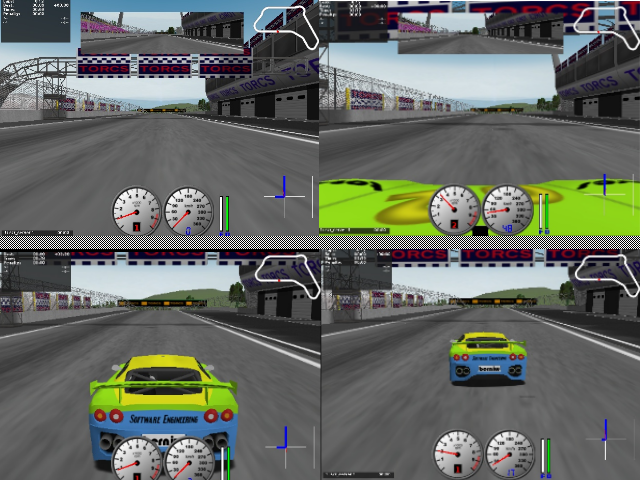
\includegraphics[width=\columnwidth]{attachments/car_view_compilation.png}
	\caption{Different camera perspectives provided by TORCS}
	\label{fig:car_views}
\end{figure}

\begin{figure}[ht]
	\centering
	\fbox{\rule{0pt}{2cm} \rule{1.0\linewidth}{0pt}}
	\caption{Mean absolute error of the same DNN trained with multiple camera angles}
	\label{fig:camera-evaluation}
\end{figure}

\subsubsection{Choosing the image size}
The images are provided by TORCS ROS \cite{mirus_torcs-ros_2017} at a rate of 10 frames per second (fps) at a resoultion of $ \SI{640}{\px} \times \SI{480}{\px} $. Because that image size is too large
to train a reasonably deep network in a reasonable time, the images are down-scaled prior to training as well as in the final application. To determine the image providing the best result, four different sizes were evaluated with the DNN described in \autoref{ssc:testing-dnn}: 
\begin{enumerate}
	\item $ \SI{320}{\px} \times \SI{240}{\px} $
	\item $ \SI{160}{\px} \times \SI{120}{\px} $
	\item $ \SI{80}{\px} \times \SI{60}{\px} $
	%\item $ \SI{40}{\px} \times \SI{30}{\px} $
\end{enumerate}
First, the training images were collected from TORCS ROS at a resolution of $ \SI{640}{\px}\times \SI{480}{\px}$. Upon loading the images, \texttt{openCV} based downscaling was applied using the bilinear interpolation algorithm. Second, the testing DNN was trained with the images at the mentioned resolutions and the mean absolute error 
for the validation set was recorded, which is visualised in \autoref{fig:img-res-evaluation}.
\begin{figure}[ht]
	\centering
	%%% Creator: Matplotlib, PGF backend
%%
%% To include the figure in your LaTeX document, write
%%   \input{<filename>.pgf}
%%
%% Make sure the required packages are loaded in your preamble
%%   \usepackage{pgf}
%%
%% Figures using additional raster images can only be included by \input if
%% they are in the same directory as the main LaTeX file. For loading figures
%% from other directories you can use the `import` package
%%   \usepackage{import}
%% and then include the figures with
%%   \import{<path to file>}{<filename>.pgf}
%%
%% Matplotlib used the following preamble
%%   \usepackage[utf8x]{inputenc}
%%   \usepackage[T1]{fontenc}
%%
\begingroup%
\makeatletter%
\begin{pgfpicture}%
\pgfpathrectangle{\pgfpointorigin}{\pgfqpoint{6.376090in}{3.940640in}}%
\pgfusepath{use as bounding box, clip}%
\begin{pgfscope}%
\pgfsetbuttcap%
\pgfsetmiterjoin%
\definecolor{currentfill}{rgb}{1.000000,1.000000,1.000000}%
\pgfsetfillcolor{currentfill}%
\pgfsetlinewidth{0.000000pt}%
\definecolor{currentstroke}{rgb}{1.000000,1.000000,1.000000}%
\pgfsetstrokecolor{currentstroke}%
\pgfsetdash{}{0pt}%
\pgfpathmoveto{\pgfqpoint{0.000000in}{0.000000in}}%
\pgfpathlineto{\pgfqpoint{6.376090in}{0.000000in}}%
\pgfpathlineto{\pgfqpoint{6.376090in}{3.940640in}}%
\pgfpathlineto{\pgfqpoint{0.000000in}{3.940640in}}%
\pgfpathclose%
\pgfusepath{fill}%
\end{pgfscope}%
\begin{pgfscope}%
\pgfsetbuttcap%
\pgfsetmiterjoin%
\definecolor{currentfill}{rgb}{1.000000,1.000000,1.000000}%
\pgfsetfillcolor{currentfill}%
\pgfsetlinewidth{0.000000pt}%
\definecolor{currentstroke}{rgb}{0.000000,0.000000,0.000000}%
\pgfsetstrokecolor{currentstroke}%
\pgfsetstrokeopacity{0.000000}%
\pgfsetdash{}{0pt}%
\pgfpathmoveto{\pgfqpoint{0.854410in}{0.524170in}}%
\pgfpathlineto{\pgfqpoint{6.191090in}{0.524170in}}%
\pgfpathlineto{\pgfqpoint{6.191090in}{3.591999in}}%
\pgfpathlineto{\pgfqpoint{0.854410in}{3.591999in}}%
\pgfpathclose%
\pgfusepath{fill}%
\end{pgfscope}%
\begin{pgfscope}%
\pgfsetbuttcap%
\pgfsetroundjoin%
\definecolor{currentfill}{rgb}{0.000000,0.000000,0.000000}%
\pgfsetfillcolor{currentfill}%
\pgfsetlinewidth{0.803000pt}%
\definecolor{currentstroke}{rgb}{0.000000,0.000000,0.000000}%
\pgfsetstrokecolor{currentstroke}%
\pgfsetdash{}{0pt}%
\pgfsys@defobject{currentmarker}{\pgfqpoint{0.000000in}{-0.048611in}}{\pgfqpoint{0.000000in}{0.000000in}}{%
\pgfpathmoveto{\pgfqpoint{0.000000in}{0.000000in}}%
\pgfpathlineto{\pgfqpoint{0.000000in}{-0.048611in}}%
\pgfusepath{stroke,fill}%
}%
\begin{pgfscope}%
\pgfsys@transformshift{1.096986in}{0.524170in}%
\pgfsys@useobject{currentmarker}{}%
\end{pgfscope}%
\end{pgfscope}%
\begin{pgfscope}%
\pgftext[x=1.096986in,y=0.426948in,,top]{\rmfamily\fontsize{8.000000}{9.600000}\selectfont \(\displaystyle 0\)}%
\end{pgfscope}%
\begin{pgfscope}%
\pgfsetbuttcap%
\pgfsetroundjoin%
\definecolor{currentfill}{rgb}{0.000000,0.000000,0.000000}%
\pgfsetfillcolor{currentfill}%
\pgfsetlinewidth{0.803000pt}%
\definecolor{currentstroke}{rgb}{0.000000,0.000000,0.000000}%
\pgfsetstrokecolor{currentstroke}%
\pgfsetdash{}{0pt}%
\pgfsys@defobject{currentmarker}{\pgfqpoint{0.000000in}{-0.048611in}}{\pgfqpoint{0.000000in}{0.000000in}}{%
\pgfpathmoveto{\pgfqpoint{0.000000in}{0.000000in}}%
\pgfpathlineto{\pgfqpoint{0.000000in}{-0.048611in}}%
\pgfusepath{stroke,fill}%
}%
\begin{pgfscope}%
\pgfsys@transformshift{1.855037in}{0.524170in}%
\pgfsys@useobject{currentmarker}{}%
\end{pgfscope}%
\end{pgfscope}%
\begin{pgfscope}%
\pgftext[x=1.855037in,y=0.426948in,,top]{\rmfamily\fontsize{8.000000}{9.600000}\selectfont \(\displaystyle 10\)}%
\end{pgfscope}%
\begin{pgfscope}%
\pgfsetbuttcap%
\pgfsetroundjoin%
\definecolor{currentfill}{rgb}{0.000000,0.000000,0.000000}%
\pgfsetfillcolor{currentfill}%
\pgfsetlinewidth{0.803000pt}%
\definecolor{currentstroke}{rgb}{0.000000,0.000000,0.000000}%
\pgfsetstrokecolor{currentstroke}%
\pgfsetdash{}{0pt}%
\pgfsys@defobject{currentmarker}{\pgfqpoint{0.000000in}{-0.048611in}}{\pgfqpoint{0.000000in}{0.000000in}}{%
\pgfpathmoveto{\pgfqpoint{0.000000in}{0.000000in}}%
\pgfpathlineto{\pgfqpoint{0.000000in}{-0.048611in}}%
\pgfusepath{stroke,fill}%
}%
\begin{pgfscope}%
\pgfsys@transformshift{2.613088in}{0.524170in}%
\pgfsys@useobject{currentmarker}{}%
\end{pgfscope}%
\end{pgfscope}%
\begin{pgfscope}%
\pgftext[x=2.613088in,y=0.426948in,,top]{\rmfamily\fontsize{8.000000}{9.600000}\selectfont \(\displaystyle 20\)}%
\end{pgfscope}%
\begin{pgfscope}%
\pgfsetbuttcap%
\pgfsetroundjoin%
\definecolor{currentfill}{rgb}{0.000000,0.000000,0.000000}%
\pgfsetfillcolor{currentfill}%
\pgfsetlinewidth{0.803000pt}%
\definecolor{currentstroke}{rgb}{0.000000,0.000000,0.000000}%
\pgfsetstrokecolor{currentstroke}%
\pgfsetdash{}{0pt}%
\pgfsys@defobject{currentmarker}{\pgfqpoint{0.000000in}{-0.048611in}}{\pgfqpoint{0.000000in}{0.000000in}}{%
\pgfpathmoveto{\pgfqpoint{0.000000in}{0.000000in}}%
\pgfpathlineto{\pgfqpoint{0.000000in}{-0.048611in}}%
\pgfusepath{stroke,fill}%
}%
\begin{pgfscope}%
\pgfsys@transformshift{3.371139in}{0.524170in}%
\pgfsys@useobject{currentmarker}{}%
\end{pgfscope}%
\end{pgfscope}%
\begin{pgfscope}%
\pgftext[x=3.371139in,y=0.426948in,,top]{\rmfamily\fontsize{8.000000}{9.600000}\selectfont \(\displaystyle 30\)}%
\end{pgfscope}%
\begin{pgfscope}%
\pgfsetbuttcap%
\pgfsetroundjoin%
\definecolor{currentfill}{rgb}{0.000000,0.000000,0.000000}%
\pgfsetfillcolor{currentfill}%
\pgfsetlinewidth{0.803000pt}%
\definecolor{currentstroke}{rgb}{0.000000,0.000000,0.000000}%
\pgfsetstrokecolor{currentstroke}%
\pgfsetdash{}{0pt}%
\pgfsys@defobject{currentmarker}{\pgfqpoint{0.000000in}{-0.048611in}}{\pgfqpoint{0.000000in}{0.000000in}}{%
\pgfpathmoveto{\pgfqpoint{0.000000in}{0.000000in}}%
\pgfpathlineto{\pgfqpoint{0.000000in}{-0.048611in}}%
\pgfusepath{stroke,fill}%
}%
\begin{pgfscope}%
\pgfsys@transformshift{4.129191in}{0.524170in}%
\pgfsys@useobject{currentmarker}{}%
\end{pgfscope}%
\end{pgfscope}%
\begin{pgfscope}%
\pgftext[x=4.129191in,y=0.426948in,,top]{\rmfamily\fontsize{8.000000}{9.600000}\selectfont \(\displaystyle 40\)}%
\end{pgfscope}%
\begin{pgfscope}%
\pgfsetbuttcap%
\pgfsetroundjoin%
\definecolor{currentfill}{rgb}{0.000000,0.000000,0.000000}%
\pgfsetfillcolor{currentfill}%
\pgfsetlinewidth{0.803000pt}%
\definecolor{currentstroke}{rgb}{0.000000,0.000000,0.000000}%
\pgfsetstrokecolor{currentstroke}%
\pgfsetdash{}{0pt}%
\pgfsys@defobject{currentmarker}{\pgfqpoint{0.000000in}{-0.048611in}}{\pgfqpoint{0.000000in}{0.000000in}}{%
\pgfpathmoveto{\pgfqpoint{0.000000in}{0.000000in}}%
\pgfpathlineto{\pgfqpoint{0.000000in}{-0.048611in}}%
\pgfusepath{stroke,fill}%
}%
\begin{pgfscope}%
\pgfsys@transformshift{4.887242in}{0.524170in}%
\pgfsys@useobject{currentmarker}{}%
\end{pgfscope}%
\end{pgfscope}%
\begin{pgfscope}%
\pgftext[x=4.887242in,y=0.426948in,,top]{\rmfamily\fontsize{8.000000}{9.600000}\selectfont \(\displaystyle 50\)}%
\end{pgfscope}%
\begin{pgfscope}%
\pgfsetbuttcap%
\pgfsetroundjoin%
\definecolor{currentfill}{rgb}{0.000000,0.000000,0.000000}%
\pgfsetfillcolor{currentfill}%
\pgfsetlinewidth{0.803000pt}%
\definecolor{currentstroke}{rgb}{0.000000,0.000000,0.000000}%
\pgfsetstrokecolor{currentstroke}%
\pgfsetdash{}{0pt}%
\pgfsys@defobject{currentmarker}{\pgfqpoint{0.000000in}{-0.048611in}}{\pgfqpoint{0.000000in}{0.000000in}}{%
\pgfpathmoveto{\pgfqpoint{0.000000in}{0.000000in}}%
\pgfpathlineto{\pgfqpoint{0.000000in}{-0.048611in}}%
\pgfusepath{stroke,fill}%
}%
\begin{pgfscope}%
\pgfsys@transformshift{5.645293in}{0.524170in}%
\pgfsys@useobject{currentmarker}{}%
\end{pgfscope}%
\end{pgfscope}%
\begin{pgfscope}%
\pgftext[x=5.645293in,y=0.426948in,,top]{\rmfamily\fontsize{8.000000}{9.600000}\selectfont \(\displaystyle 60\)}%
\end{pgfscope}%
\begin{pgfscope}%
\pgftext[x=3.522750in,y=0.273268in,,top]{\rmfamily\fontsize{10.000000}{12.000000}\selectfont num epochs}%
\end{pgfscope}%
\begin{pgfscope}%
\pgfsetbuttcap%
\pgfsetroundjoin%
\definecolor{currentfill}{rgb}{0.000000,0.000000,0.000000}%
\pgfsetfillcolor{currentfill}%
\pgfsetlinewidth{0.602250pt}%
\definecolor{currentstroke}{rgb}{0.000000,0.000000,0.000000}%
\pgfsetstrokecolor{currentstroke}%
\pgfsetdash{}{0pt}%
\pgfsys@defobject{currentmarker}{\pgfqpoint{-0.027778in}{0.000000in}}{\pgfqpoint{0.000000in}{0.000000in}}{%
\pgfpathmoveto{\pgfqpoint{0.000000in}{0.000000in}}%
\pgfpathlineto{\pgfqpoint{-0.027778in}{0.000000in}}%
\pgfusepath{stroke,fill}%
}%
\begin{pgfscope}%
\pgfsys@transformshift{0.854410in}{1.279515in}%
\pgfsys@useobject{currentmarker}{}%
\end{pgfscope}%
\end{pgfscope}%
\begin{pgfscope}%
\pgftext[x=0.319916in,y=1.234597in,left,base]{\rmfamily\fontsize{8.000000}{9.600000}\selectfont \(\displaystyle 4\times10^{-2}\)}%
\end{pgfscope}%
\begin{pgfscope}%
\pgfsetbuttcap%
\pgfsetroundjoin%
\definecolor{currentfill}{rgb}{0.000000,0.000000,0.000000}%
\pgfsetfillcolor{currentfill}%
\pgfsetlinewidth{0.602250pt}%
\definecolor{currentstroke}{rgb}{0.000000,0.000000,0.000000}%
\pgfsetstrokecolor{currentstroke}%
\pgfsetdash{}{0pt}%
\pgfsys@defobject{currentmarker}{\pgfqpoint{-0.027778in}{0.000000in}}{\pgfqpoint{0.000000in}{0.000000in}}{%
\pgfpathmoveto{\pgfqpoint{0.000000in}{0.000000in}}%
\pgfpathlineto{\pgfqpoint{-0.027778in}{0.000000in}}%
\pgfusepath{stroke,fill}%
}%
\begin{pgfscope}%
\pgfsys@transformshift{0.854410in}{2.182696in}%
\pgfsys@useobject{currentmarker}{}%
\end{pgfscope}%
\end{pgfscope}%
\begin{pgfscope}%
\pgftext[x=0.319916in,y=2.137778in,left,base]{\rmfamily\fontsize{8.000000}{9.600000}\selectfont \(\displaystyle 5\times10^{-2}\)}%
\end{pgfscope}%
\begin{pgfscope}%
\pgfsetbuttcap%
\pgfsetroundjoin%
\definecolor{currentfill}{rgb}{0.000000,0.000000,0.000000}%
\pgfsetfillcolor{currentfill}%
\pgfsetlinewidth{0.602250pt}%
\definecolor{currentstroke}{rgb}{0.000000,0.000000,0.000000}%
\pgfsetstrokecolor{currentstroke}%
\pgfsetdash{}{0pt}%
\pgfsys@defobject{currentmarker}{\pgfqpoint{-0.027778in}{0.000000in}}{\pgfqpoint{0.000000in}{0.000000in}}{%
\pgfpathmoveto{\pgfqpoint{0.000000in}{0.000000in}}%
\pgfpathlineto{\pgfqpoint{-0.027778in}{0.000000in}}%
\pgfusepath{stroke,fill}%
}%
\begin{pgfscope}%
\pgfsys@transformshift{0.854410in}{2.920648in}%
\pgfsys@useobject{currentmarker}{}%
\end{pgfscope}%
\end{pgfscope}%
\begin{pgfscope}%
\pgftext[x=0.319916in,y=2.875730in,left,base]{\rmfamily\fontsize{8.000000}{9.600000}\selectfont \(\displaystyle 6\times10^{-2}\)}%
\end{pgfscope}%
\begin{pgfscope}%
\pgfsetbuttcap%
\pgfsetroundjoin%
\definecolor{currentfill}{rgb}{0.000000,0.000000,0.000000}%
\pgfsetfillcolor{currentfill}%
\pgfsetlinewidth{0.602250pt}%
\definecolor{currentstroke}{rgb}{0.000000,0.000000,0.000000}%
\pgfsetstrokecolor{currentstroke}%
\pgfsetdash{}{0pt}%
\pgfsys@defobject{currentmarker}{\pgfqpoint{-0.027778in}{0.000000in}}{\pgfqpoint{0.000000in}{0.000000in}}{%
\pgfpathmoveto{\pgfqpoint{0.000000in}{0.000000in}}%
\pgfpathlineto{\pgfqpoint{-0.027778in}{0.000000in}}%
\pgfusepath{stroke,fill}%
}%
\begin{pgfscope}%
\pgfsys@transformshift{0.854410in}{3.544578in}%
\pgfsys@useobject{currentmarker}{}%
\end{pgfscope}%
\end{pgfscope}%
\begin{pgfscope}%
\pgftext[x=0.319916in,y=3.499660in,left,base]{\rmfamily\fontsize{8.000000}{9.600000}\selectfont \(\displaystyle 7\times10^{-2}\)}%
\end{pgfscope}%
\begin{pgfscope}%
\pgftext[x=0.264360in,y=2.058084in,,bottom,rotate=90.000000]{\rmfamily\fontsize{10.000000}{12.000000}\selectfont mae}%
\end{pgfscope}%
\begin{pgfscope}%
\pgfpathrectangle{\pgfqpoint{0.854410in}{0.524170in}}{\pgfqpoint{5.336680in}{3.067829in}} %
\pgfusepath{clip}%
\pgfsetrectcap%
\pgfsetroundjoin%
\pgfsetlinewidth{1.505625pt}%
\definecolor{currentstroke}{rgb}{0.121569,0.466667,0.705882}%
\pgfsetstrokecolor{currentstroke}%
\pgfsetdash{}{0pt}%
\pgfpathmoveto{\pgfqpoint{1.096986in}{2.660354in}}%
\pgfpathlineto{\pgfqpoint{1.172791in}{1.925819in}}%
\pgfpathlineto{\pgfqpoint{1.248596in}{1.718483in}}%
\pgfpathlineto{\pgfqpoint{1.324401in}{3.069358in}}%
\pgfpathlineto{\pgfqpoint{1.400207in}{1.685475in}}%
\pgfpathlineto{\pgfqpoint{1.476012in}{1.639951in}}%
\pgfpathlineto{\pgfqpoint{1.551817in}{1.528252in}}%
\pgfpathlineto{\pgfqpoint{1.627622in}{1.519144in}}%
\pgfpathlineto{\pgfqpoint{1.703427in}{1.895035in}}%
\pgfpathlineto{\pgfqpoint{1.779232in}{2.111485in}}%
\pgfpathlineto{\pgfqpoint{1.855037in}{1.272586in}}%
\pgfpathlineto{\pgfqpoint{1.930842in}{1.229227in}}%
\pgfpathlineto{\pgfqpoint{2.006647in}{1.498268in}}%
\pgfpathlineto{\pgfqpoint{2.082453in}{1.430874in}}%
\pgfpathlineto{\pgfqpoint{2.158258in}{1.227377in}}%
\pgfpathlineto{\pgfqpoint{2.234063in}{1.045520in}}%
\pgfpathlineto{\pgfqpoint{2.309868in}{1.008931in}}%
\pgfpathlineto{\pgfqpoint{2.385673in}{1.277476in}}%
\pgfpathlineto{\pgfqpoint{2.461478in}{1.120360in}}%
\pgfpathlineto{\pgfqpoint{2.537283in}{1.249820in}}%
\pgfpathlineto{\pgfqpoint{2.613088in}{0.824144in}}%
\pgfpathlineto{\pgfqpoint{2.688893in}{1.237605in}}%
\pgfpathlineto{\pgfqpoint{2.764699in}{1.594019in}}%
\pgfpathlineto{\pgfqpoint{2.840504in}{1.625030in}}%
\pgfpathlineto{\pgfqpoint{2.916309in}{1.196789in}}%
\pgfpathlineto{\pgfqpoint{2.992114in}{1.197478in}}%
\pgfpathlineto{\pgfqpoint{3.067919in}{1.145366in}}%
\pgfpathlineto{\pgfqpoint{3.143724in}{1.489282in}}%
\pgfpathlineto{\pgfqpoint{3.219529in}{1.390704in}}%
\pgfpathlineto{\pgfqpoint{3.295334in}{1.832679in}}%
\pgfpathlineto{\pgfqpoint{3.371139in}{0.990454in}}%
\pgfpathlineto{\pgfqpoint{3.446945in}{1.033596in}}%
\pgfpathlineto{\pgfqpoint{3.522750in}{1.025963in}}%
\pgfpathlineto{\pgfqpoint{3.598555in}{0.923950in}}%
\pgfpathlineto{\pgfqpoint{3.674360in}{0.778092in}}%
\pgfpathlineto{\pgfqpoint{3.750165in}{0.789609in}}%
\pgfpathlineto{\pgfqpoint{3.825970in}{0.855179in}}%
\pgfpathlineto{\pgfqpoint{3.901775in}{0.993374in}}%
\pgfpathlineto{\pgfqpoint{3.977580in}{0.773715in}}%
\pgfpathlineto{\pgfqpoint{4.053385in}{2.622004in}}%
\pgfpathlineto{\pgfqpoint{4.129191in}{0.954998in}}%
\pgfpathlineto{\pgfqpoint{4.204996in}{0.821253in}}%
\pgfpathlineto{\pgfqpoint{4.280801in}{0.843650in}}%
\pgfpathlineto{\pgfqpoint{4.356606in}{1.342733in}}%
\pgfpathlineto{\pgfqpoint{4.432411in}{0.736728in}}%
\pgfpathlineto{\pgfqpoint{4.508216in}{0.678212in}}%
\pgfpathlineto{\pgfqpoint{4.584021in}{1.635107in}}%
\pgfpathlineto{\pgfqpoint{4.659826in}{1.219532in}}%
\pgfpathlineto{\pgfqpoint{4.735632in}{0.912959in}}%
\pgfpathlineto{\pgfqpoint{4.811437in}{0.862746in}}%
\pgfpathlineto{\pgfqpoint{4.887242in}{1.071581in}}%
\pgfpathlineto{\pgfqpoint{4.963047in}{0.665202in}}%
\pgfpathlineto{\pgfqpoint{5.038852in}{0.853209in}}%
\pgfpathlineto{\pgfqpoint{5.114657in}{0.791867in}}%
\pgfpathlineto{\pgfqpoint{5.190462in}{0.663617in}}%
\pgfpathlineto{\pgfqpoint{5.266267in}{0.894700in}}%
\pgfpathlineto{\pgfqpoint{5.342072in}{0.840689in}}%
\pgfpathlineto{\pgfqpoint{5.417878in}{0.679089in}}%
\pgfpathlineto{\pgfqpoint{5.493683in}{0.774084in}}%
\pgfpathlineto{\pgfqpoint{5.569488in}{0.688450in}}%
\pgfpathlineto{\pgfqpoint{5.645293in}{0.757420in}}%
\pgfpathlineto{\pgfqpoint{5.721098in}{0.971099in}}%
\pgfpathlineto{\pgfqpoint{5.796903in}{1.053366in}}%
\pgfpathlineto{\pgfqpoint{5.872708in}{1.071472in}}%
\pgfpathlineto{\pgfqpoint{5.948513in}{0.681855in}}%
\pgfusepath{stroke}%
\end{pgfscope}%
\begin{pgfscope}%
\pgfpathrectangle{\pgfqpoint{0.854410in}{0.524170in}}{\pgfqpoint{5.336680in}{3.067829in}} %
\pgfusepath{clip}%
\pgfsetrectcap%
\pgfsetroundjoin%
\pgfsetlinewidth{1.505625pt}%
\definecolor{currentstroke}{rgb}{1.000000,0.498039,0.054902}%
\pgfsetstrokecolor{currentstroke}%
\pgfsetdash{}{0pt}%
\pgfpathmoveto{\pgfqpoint{1.096986in}{3.351819in}}%
\pgfpathlineto{\pgfqpoint{1.172791in}{3.184270in}}%
\pgfpathlineto{\pgfqpoint{1.248596in}{2.606518in}}%
\pgfpathlineto{\pgfqpoint{1.324401in}{2.571192in}}%
\pgfpathlineto{\pgfqpoint{1.400207in}{2.605360in}}%
\pgfpathlineto{\pgfqpoint{1.476012in}{3.452552in}}%
\pgfpathlineto{\pgfqpoint{1.551817in}{3.002201in}}%
\pgfpathlineto{\pgfqpoint{1.627622in}{2.789026in}}%
\pgfpathlineto{\pgfqpoint{1.703427in}{2.506142in}}%
\pgfpathlineto{\pgfqpoint{1.779232in}{2.950306in}}%
\pgfpathlineto{\pgfqpoint{1.855037in}{2.450082in}}%
\pgfpathlineto{\pgfqpoint{1.930842in}{2.327692in}}%
\pgfpathlineto{\pgfqpoint{2.006647in}{1.998345in}}%
\pgfpathlineto{\pgfqpoint{2.082453in}{2.120532in}}%
\pgfpathlineto{\pgfqpoint{2.158258in}{1.805315in}}%
\pgfpathlineto{\pgfqpoint{2.234063in}{2.231156in}}%
\pgfpathlineto{\pgfqpoint{2.309868in}{1.886762in}}%
\pgfpathlineto{\pgfqpoint{2.385673in}{1.979167in}}%
\pgfpathlineto{\pgfqpoint{2.461478in}{2.037710in}}%
\pgfpathlineto{\pgfqpoint{2.537283in}{1.755632in}}%
\pgfpathlineto{\pgfqpoint{2.613088in}{2.195681in}}%
\pgfpathlineto{\pgfqpoint{2.688893in}{2.540911in}}%
\pgfpathlineto{\pgfqpoint{2.764699in}{2.001154in}}%
\pgfpathlineto{\pgfqpoint{2.840504in}{1.740617in}}%
\pgfpathlineto{\pgfqpoint{2.916309in}{1.744179in}}%
\pgfpathlineto{\pgfqpoint{2.992114in}{2.235963in}}%
\pgfpathlineto{\pgfqpoint{3.067919in}{1.849547in}}%
\pgfpathlineto{\pgfqpoint{3.143724in}{1.897300in}}%
\pgfpathlineto{\pgfqpoint{3.219529in}{2.107552in}}%
\pgfpathlineto{\pgfqpoint{3.295334in}{2.714119in}}%
\pgfpathlineto{\pgfqpoint{3.371139in}{1.710785in}}%
\pgfpathlineto{\pgfqpoint{3.446945in}{1.910090in}}%
\pgfpathlineto{\pgfqpoint{3.522750in}{2.167408in}}%
\pgfpathlineto{\pgfqpoint{3.598555in}{1.793140in}}%
\pgfpathlineto{\pgfqpoint{3.674360in}{1.662235in}}%
\pgfpathlineto{\pgfqpoint{3.750165in}{1.696144in}}%
\pgfpathlineto{\pgfqpoint{3.825970in}{1.802289in}}%
\pgfpathlineto{\pgfqpoint{3.901775in}{1.820367in}}%
\pgfpathlineto{\pgfqpoint{3.977580in}{1.600706in}}%
\pgfpathlineto{\pgfqpoint{4.053385in}{1.609226in}}%
\pgfpathlineto{\pgfqpoint{4.129191in}{2.060640in}}%
\pgfpathlineto{\pgfqpoint{4.204996in}{2.005149in}}%
\pgfpathlineto{\pgfqpoint{4.280801in}{1.631652in}}%
\pgfpathlineto{\pgfqpoint{4.356606in}{1.823155in}}%
\pgfpathlineto{\pgfqpoint{4.432411in}{1.720527in}}%
\pgfpathlineto{\pgfqpoint{4.508216in}{2.034173in}}%
\pgfpathlineto{\pgfqpoint{4.584021in}{1.749224in}}%
\pgfpathlineto{\pgfqpoint{4.659826in}{2.010100in}}%
\pgfpathlineto{\pgfqpoint{4.735632in}{1.854502in}}%
\pgfpathlineto{\pgfqpoint{4.811437in}{1.666254in}}%
\pgfpathlineto{\pgfqpoint{4.887242in}{1.548976in}}%
\pgfpathlineto{\pgfqpoint{4.963047in}{1.608199in}}%
\pgfpathlineto{\pgfqpoint{5.038852in}{2.074670in}}%
\pgfpathlineto{\pgfqpoint{5.114657in}{2.111722in}}%
\pgfpathlineto{\pgfqpoint{5.190462in}{1.558314in}}%
\pgfpathlineto{\pgfqpoint{5.266267in}{1.559367in}}%
\pgfpathlineto{\pgfqpoint{5.342072in}{1.665508in}}%
\pgfpathlineto{\pgfqpoint{5.417878in}{1.572742in}}%
\pgfpathlineto{\pgfqpoint{5.493683in}{1.597401in}}%
\pgfpathlineto{\pgfqpoint{5.569488in}{2.059344in}}%
\pgfpathlineto{\pgfqpoint{5.645293in}{1.767284in}}%
\pgfpathlineto{\pgfqpoint{5.721098in}{1.685185in}}%
\pgfpathlineto{\pgfqpoint{5.796903in}{1.808485in}}%
\pgfpathlineto{\pgfqpoint{5.872708in}{1.646152in}}%
\pgfpathlineto{\pgfqpoint{5.948513in}{2.303404in}}%
\pgfusepath{stroke}%
\end{pgfscope}%
\begin{pgfscope}%
\pgfpathrectangle{\pgfqpoint{0.854410in}{0.524170in}}{\pgfqpoint{5.336680in}{3.067829in}} %
\pgfusepath{clip}%
\pgfsetrectcap%
\pgfsetroundjoin%
\pgfsetlinewidth{1.505625pt}%
\definecolor{currentstroke}{rgb}{0.172549,0.627451,0.172549}%
\pgfsetstrokecolor{currentstroke}%
\pgfsetdash{}{0pt}%
\pgfpathmoveto{\pgfqpoint{1.096986in}{2.953682in}}%
\pgfpathlineto{\pgfqpoint{1.172791in}{3.246636in}}%
\pgfpathlineto{\pgfqpoint{1.248596in}{3.052315in}}%
\pgfpathlineto{\pgfqpoint{1.324401in}{2.575649in}}%
\pgfpathlineto{\pgfqpoint{1.400207in}{2.687102in}}%
\pgfpathlineto{\pgfqpoint{1.476012in}{2.411825in}}%
\pgfpathlineto{\pgfqpoint{1.551817in}{2.521504in}}%
\pgfpathlineto{\pgfqpoint{1.627622in}{2.715229in}}%
\pgfpathlineto{\pgfqpoint{1.703427in}{1.403587in}}%
\pgfpathlineto{\pgfqpoint{1.779232in}{1.028855in}}%
\pgfpathlineto{\pgfqpoint{1.855037in}{1.548981in}}%
\pgfpathlineto{\pgfqpoint{1.930842in}{2.572311in}}%
\pgfpathlineto{\pgfqpoint{2.006647in}{1.144489in}}%
\pgfpathlineto{\pgfqpoint{2.082453in}{1.543287in}}%
\pgfpathlineto{\pgfqpoint{2.158258in}{2.969316in}}%
\pgfpathlineto{\pgfqpoint{2.234063in}{2.965509in}}%
\pgfpathlineto{\pgfqpoint{2.309868in}{3.002880in}}%
\pgfpathlineto{\pgfqpoint{2.385673in}{3.040677in}}%
\pgfpathlineto{\pgfqpoint{2.461478in}{3.086818in}}%
\pgfpathlineto{\pgfqpoint{2.537283in}{3.028110in}}%
\pgfpathlineto{\pgfqpoint{2.613088in}{3.061204in}}%
\pgfpathlineto{\pgfqpoint{2.688893in}{3.014030in}}%
\pgfpathlineto{\pgfqpoint{2.764699in}{3.027925in}}%
\pgfpathlineto{\pgfqpoint{2.840504in}{3.012163in}}%
\pgfpathlineto{\pgfqpoint{2.916309in}{3.026879in}}%
\pgfpathlineto{\pgfqpoint{2.992114in}{3.056261in}}%
\pgfpathlineto{\pgfqpoint{3.067919in}{3.008355in}}%
\pgfpathlineto{\pgfqpoint{3.143724in}{3.012004in}}%
\pgfpathlineto{\pgfqpoint{3.219529in}{2.991651in}}%
\pgfpathlineto{\pgfqpoint{3.295334in}{2.971655in}}%
\pgfpathlineto{\pgfqpoint{3.371139in}{3.028701in}}%
\pgfpathlineto{\pgfqpoint{3.446945in}{3.006190in}}%
\pgfpathlineto{\pgfqpoint{3.522750in}{3.013904in}}%
\pgfpathlineto{\pgfqpoint{3.598555in}{3.007251in}}%
\pgfpathlineto{\pgfqpoint{3.674360in}{3.083997in}}%
\pgfpathlineto{\pgfqpoint{3.750165in}{3.015602in}}%
\pgfpathlineto{\pgfqpoint{3.825970in}{3.026563in}}%
\pgfpathlineto{\pgfqpoint{3.901775in}{3.012523in}}%
\pgfpathlineto{\pgfqpoint{3.977580in}{3.050855in}}%
\pgfpathlineto{\pgfqpoint{4.053385in}{2.989608in}}%
\pgfpathlineto{\pgfqpoint{4.129191in}{3.040286in}}%
\pgfpathlineto{\pgfqpoint{4.204996in}{3.039478in}}%
\pgfpathlineto{\pgfqpoint{4.280801in}{2.982896in}}%
\pgfpathlineto{\pgfqpoint{4.356606in}{2.994202in}}%
\pgfpathlineto{\pgfqpoint{4.432411in}{3.024241in}}%
\pgfpathlineto{\pgfqpoint{4.508216in}{3.023904in}}%
\pgfpathlineto{\pgfqpoint{4.584021in}{3.047694in}}%
\pgfpathlineto{\pgfqpoint{4.659826in}{3.023010in}}%
\pgfpathlineto{\pgfqpoint{4.735632in}{3.040936in}}%
\pgfpathlineto{\pgfqpoint{4.811437in}{3.019328in}}%
\pgfpathlineto{\pgfqpoint{4.887242in}{3.003249in}}%
\pgfpathlineto{\pgfqpoint{4.963047in}{3.023043in}}%
\pgfpathlineto{\pgfqpoint{5.038852in}{3.000945in}}%
\pgfpathlineto{\pgfqpoint{5.114657in}{3.011015in}}%
\pgfpathlineto{\pgfqpoint{5.190462in}{3.014357in}}%
\pgfpathlineto{\pgfqpoint{5.266267in}{3.050261in}}%
\pgfpathlineto{\pgfqpoint{5.342072in}{3.010974in}}%
\pgfpathlineto{\pgfqpoint{5.417878in}{3.087060in}}%
\pgfpathlineto{\pgfqpoint{5.493683in}{2.980018in}}%
\pgfpathlineto{\pgfqpoint{5.569488in}{3.029121in}}%
\pgfpathlineto{\pgfqpoint{5.645293in}{3.044940in}}%
\pgfpathlineto{\pgfqpoint{5.721098in}{3.093198in}}%
\pgfpathlineto{\pgfqpoint{5.796903in}{3.086618in}}%
\pgfpathlineto{\pgfqpoint{5.872708in}{3.052364in}}%
\pgfpathlineto{\pgfqpoint{5.948513in}{3.046837in}}%
\pgfusepath{stroke}%
\end{pgfscope}%
\begin{pgfscope}%
\pgfsetrectcap%
\pgfsetmiterjoin%
\pgfsetlinewidth{0.803000pt}%
\definecolor{currentstroke}{rgb}{0.000000,0.000000,0.000000}%
\pgfsetstrokecolor{currentstroke}%
\pgfsetdash{}{0pt}%
\pgfpathmoveto{\pgfqpoint{0.854410in}{0.524170in}}%
\pgfpathlineto{\pgfqpoint{0.854410in}{3.591999in}}%
\pgfusepath{stroke}%
\end{pgfscope}%
\begin{pgfscope}%
\pgfsetrectcap%
\pgfsetmiterjoin%
\pgfsetlinewidth{0.803000pt}%
\definecolor{currentstroke}{rgb}{0.000000,0.000000,0.000000}%
\pgfsetstrokecolor{currentstroke}%
\pgfsetdash{}{0pt}%
\pgfpathmoveto{\pgfqpoint{6.191090in}{0.524170in}}%
\pgfpathlineto{\pgfqpoint{6.191090in}{3.591999in}}%
\pgfusepath{stroke}%
\end{pgfscope}%
\begin{pgfscope}%
\pgfsetrectcap%
\pgfsetmiterjoin%
\pgfsetlinewidth{0.803000pt}%
\definecolor{currentstroke}{rgb}{0.000000,0.000000,0.000000}%
\pgfsetstrokecolor{currentstroke}%
\pgfsetdash{}{0pt}%
\pgfpathmoveto{\pgfqpoint{0.854410in}{0.524170in}}%
\pgfpathlineto{\pgfqpoint{6.191090in}{0.524170in}}%
\pgfusepath{stroke}%
\end{pgfscope}%
\begin{pgfscope}%
\pgfsetrectcap%
\pgfsetmiterjoin%
\pgfsetlinewidth{0.803000pt}%
\definecolor{currentstroke}{rgb}{0.000000,0.000000,0.000000}%
\pgfsetstrokecolor{currentstroke}%
\pgfsetdash{}{0pt}%
\pgfpathmoveto{\pgfqpoint{0.854410in}{3.591999in}}%
\pgfpathlineto{\pgfqpoint{6.191090in}{3.591999in}}%
\pgfusepath{stroke}%
\end{pgfscope}%
\begin{pgfscope}%
\pgftext[x=3.522750in,y=3.675332in,,base]{\rmfamily\fontsize{12.000000}{14.400000}\selectfont mae of DNN on map: data-olethros road 1-2laps-640x480.}%
\end{pgfscope}%
\begin{pgfscope}%
\pgfsetbuttcap%
\pgfsetmiterjoin%
\definecolor{currentfill}{rgb}{1.000000,1.000000,1.000000}%
\pgfsetfillcolor{currentfill}%
\pgfsetfillopacity{0.800000}%
\pgfsetlinewidth{1.003750pt}%
\definecolor{currentstroke}{rgb}{0.800000,0.800000,0.800000}%
\pgfsetstrokecolor{currentstroke}%
\pgfsetstrokeopacity{0.800000}%
\pgfsetdash{}{0pt}%
\pgfpathmoveto{\pgfqpoint{2.882187in}{2.761467in}}%
\pgfpathlineto{\pgfqpoint{4.163312in}{2.761467in}}%
\pgfpathquadraticcurveto{\pgfqpoint{4.196645in}{2.761467in}}{\pgfqpoint{4.196645in}{2.794800in}}%
\pgfpathlineto{\pgfqpoint{4.196645in}{3.475332in}}%
\pgfpathquadraticcurveto{\pgfqpoint{4.196645in}{3.508665in}}{\pgfqpoint{4.163312in}{3.508665in}}%
\pgfpathlineto{\pgfqpoint{2.882187in}{3.508665in}}%
\pgfpathquadraticcurveto{\pgfqpoint{2.848854in}{3.508665in}}{\pgfqpoint{2.848854in}{3.475332in}}%
\pgfpathlineto{\pgfqpoint{2.848854in}{2.794800in}}%
\pgfpathquadraticcurveto{\pgfqpoint{2.848854in}{2.761467in}}{\pgfqpoint{2.882187in}{2.761467in}}%
\pgfpathclose%
\pgfusepath{stroke,fill}%
\end{pgfscope}%
\begin{pgfscope}%
\pgfsetrectcap%
\pgfsetroundjoin%
\pgfsetlinewidth{1.505625pt}%
\definecolor{currentstroke}{rgb}{0.121569,0.466667,0.705882}%
\pgfsetstrokecolor{currentstroke}%
\pgfsetdash{}{0pt}%
\pgfpathmoveto{\pgfqpoint{2.915521in}{3.383665in}}%
\pgfpathlineto{\pgfqpoint{3.248854in}{3.383665in}}%
\pgfusepath{stroke}%
\end{pgfscope}%
\begin{pgfscope}%
\pgftext[x=3.382187in,y=3.325332in,left,base]{\rmfamily\fontsize{12.000000}{14.400000}\selectfont 80x60px}%
\end{pgfscope}%
\begin{pgfscope}%
\pgfsetrectcap%
\pgfsetroundjoin%
\pgfsetlinewidth{1.505625pt}%
\definecolor{currentstroke}{rgb}{1.000000,0.498039,0.054902}%
\pgfsetstrokecolor{currentstroke}%
\pgfsetdash{}{0pt}%
\pgfpathmoveto{\pgfqpoint{2.915521in}{3.151266in}}%
\pgfpathlineto{\pgfqpoint{3.248854in}{3.151266in}}%
\pgfusepath{stroke}%
\end{pgfscope}%
\begin{pgfscope}%
\pgftext[x=3.382187in,y=3.092933in,left,base]{\rmfamily\fontsize{12.000000}{14.400000}\selectfont 160x120px}%
\end{pgfscope}%
\begin{pgfscope}%
\pgfsetrectcap%
\pgfsetroundjoin%
\pgfsetlinewidth{1.505625pt}%
\definecolor{currentstroke}{rgb}{0.172549,0.627451,0.172549}%
\pgfsetstrokecolor{currentstroke}%
\pgfsetdash{}{0pt}%
\pgfpathmoveto{\pgfqpoint{2.915521in}{2.918867in}}%
\pgfpathlineto{\pgfqpoint{3.248854in}{2.918867in}}%
\pgfusepath{stroke}%
\end{pgfscope}%
\begin{pgfscope}%
\pgftext[x=3.382187in,y=2.860533in,left,base]{\rmfamily\fontsize{12.000000}{14.400000}\selectfont 320x240px}%
\end{pgfscope}%
\end{pgfpicture}%
\makeatother%
\endgroup%

	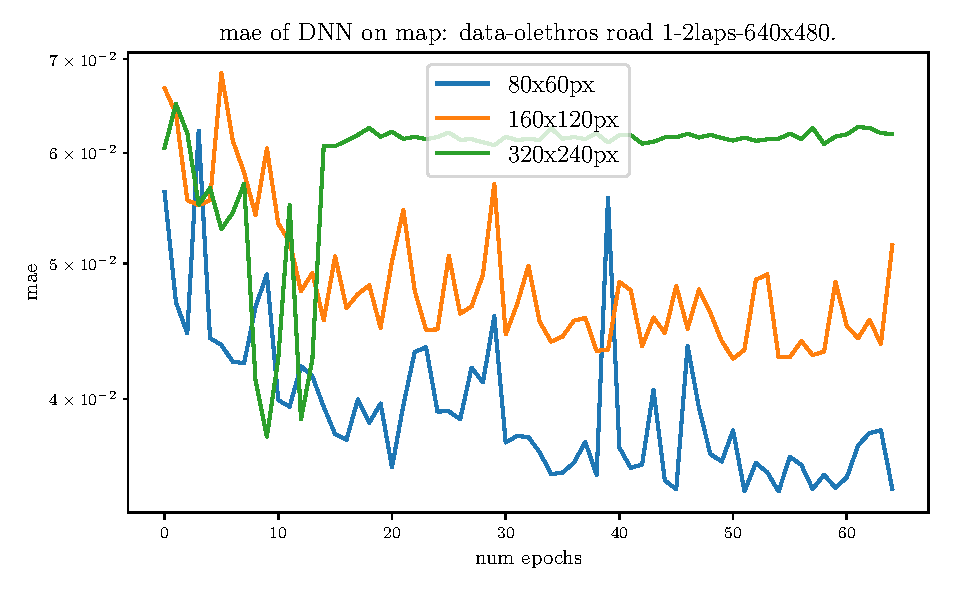
\includegraphics[width=\columnwidth]{attachments/alexnet-val_mae-img_size_compare-09042-12547-22111.pdf}
	\caption{Mean absolute error of the same DNN trained with multiple image resolutions}
	\label{fig:img-res-evaluation}
\end{figure}

Therefore, the image size $ \SI{80}{\px}\times\SI{60}{\px} $ is used for the DNN as it provides the smallest mean absolute error and additionally reduces the training time due to the small image size.

\subsection{Choosing the optimiser}
\label{sc:optimiser-choice}
A plethora of different optimisers are available for use in the backpropagation step when training DNNs. The largest differences are in their abilities to exit large local maxima, training performance and accuracy. As the currently used DNN is managable in size, the training performance is not yet a critical property. Therefore, the optimiser was selected based on its ability to minimse the mean absolute error of the validation set. As illustrated in \autoref{fig:optimiser-evaluation}, the \texttt{adamax} optimiser provides the best result and is thus chosen for future application. \texttt{adamax} is similiar to the \texttt{adam} optimiser while being more stable in certain conditions, see \cite{DBLP:journals/corr/KingmaB14} for more details. 

\begin{figure}[ht]
	\centering
	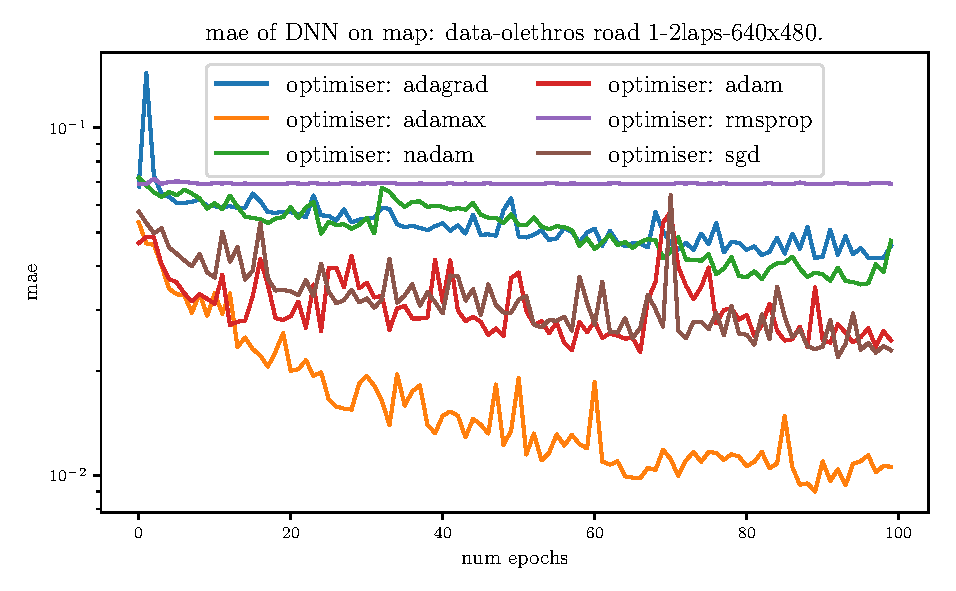
\includegraphics[width=\columnwidth]{attachments/alexnet-val_mae-optimiser_comp-69975-70890-71951-76023-79233-82251.pdf}
	\caption{Optimiser comparison in the test DNN using with an image size of $ \SI{80}{\px}\times\SI{60}{\px} $}
	\label{fig:optimiser-evaluation}
\end{figure}

\subsection{Building a deep neural network with keras}
\label{ssc:keras}
Keras is a python library 
hello keras \cite{Toshev_2014_CVPR}

\section{Nengo Controller}
\label{sc:controller}
The controller of the car is designed based on Spiking Neural Networks (SNN) which are implemented in Nengo \cite{nengo}, a python framework for building large-scale neural systems that is based on the Neural Engineering Framework (NEF) \cite{nef}. \\
The controller is divided in several modular parts: acceleration, braking, steering, gear changing and clutching. We choose the modular approach, because it allows to test different modules independently from each other and also mix hard coded solutions with learned ones.

\subsection{Nengo controller design}
In the default driver's source code, the driving modules are based on different sensor inputs. The steering module is a function based on the car speed $v_x$, the lateral displacement $d_{lat}$ and the rotation angle $\alpha$. Both, the acceleration and the braking module are based on three range sensor signals $-5$, $0$ and $5$ degrees as well as $v_x$. We chose to implement the gear changing as a hard coded solution without any learning involved, since it is a simple if-else condition. It is further possible to neglect the clutching module, because it did not show to make any difference for driver performance even though it is implemented in the default driver. The final model architecture can be seen in \autoref{fig:nengo_architecture}.\\
\begin{figure}[ht]
	\centering
	%%% Creator: Matplotlib, PGF backend
%%
%% To include the figure in your LaTeX document, write
%%   \input{<filename>.pgf}
%%
%% Make sure the required packages are loaded in your preamble
%%   \usepackage{pgf}
%%
%% Figures using additional raster images can only be included by \input if
%% they are in the same directory as the main LaTeX file. For loading figures
%% from other directories you can use the `import` package
%%   \usepackage{import}
%% and then include the figures with
%%   \import{<path to file>}{<filename>.pgf}
%%
%% Matplotlib used the following preamble
%%   \usepackage[utf8x]{inputenc}
%%   \usepackage[T1]{fontenc}
%%
\begingroup%
\makeatletter%
\begin{pgfpicture}%
\pgfpathrectangle{\pgfpointorigin}{\pgfqpoint{6.376090in}{3.940640in}}%
\pgfusepath{use as bounding box, clip}%
\begin{pgfscope}%
\pgfsetbuttcap%
\pgfsetmiterjoin%
\definecolor{currentfill}{rgb}{1.000000,1.000000,1.000000}%
\pgfsetfillcolor{currentfill}%
\pgfsetlinewidth{0.000000pt}%
\definecolor{currentstroke}{rgb}{1.000000,1.000000,1.000000}%
\pgfsetstrokecolor{currentstroke}%
\pgfsetdash{}{0pt}%
\pgfpathmoveto{\pgfqpoint{0.000000in}{0.000000in}}%
\pgfpathlineto{\pgfqpoint{6.376090in}{0.000000in}}%
\pgfpathlineto{\pgfqpoint{6.376090in}{3.940640in}}%
\pgfpathlineto{\pgfqpoint{0.000000in}{3.940640in}}%
\pgfpathclose%
\pgfusepath{fill}%
\end{pgfscope}%
\begin{pgfscope}%
\pgfsetbuttcap%
\pgfsetmiterjoin%
\definecolor{currentfill}{rgb}{1.000000,1.000000,1.000000}%
\pgfsetfillcolor{currentfill}%
\pgfsetlinewidth{0.000000pt}%
\definecolor{currentstroke}{rgb}{0.000000,0.000000,0.000000}%
\pgfsetstrokecolor{currentstroke}%
\pgfsetstrokeopacity{0.000000}%
\pgfsetdash{}{0pt}%
\pgfpathmoveto{\pgfqpoint{0.854410in}{0.524170in}}%
\pgfpathlineto{\pgfqpoint{6.191090in}{0.524170in}}%
\pgfpathlineto{\pgfqpoint{6.191090in}{3.591999in}}%
\pgfpathlineto{\pgfqpoint{0.854410in}{3.591999in}}%
\pgfpathclose%
\pgfusepath{fill}%
\end{pgfscope}%
\begin{pgfscope}%
\pgfsetbuttcap%
\pgfsetroundjoin%
\definecolor{currentfill}{rgb}{0.000000,0.000000,0.000000}%
\pgfsetfillcolor{currentfill}%
\pgfsetlinewidth{0.803000pt}%
\definecolor{currentstroke}{rgb}{0.000000,0.000000,0.000000}%
\pgfsetstrokecolor{currentstroke}%
\pgfsetdash{}{0pt}%
\pgfsys@defobject{currentmarker}{\pgfqpoint{0.000000in}{-0.048611in}}{\pgfqpoint{0.000000in}{0.000000in}}{%
\pgfpathmoveto{\pgfqpoint{0.000000in}{0.000000in}}%
\pgfpathlineto{\pgfqpoint{0.000000in}{-0.048611in}}%
\pgfusepath{stroke,fill}%
}%
\begin{pgfscope}%
\pgfsys@transformshift{1.096986in}{0.524170in}%
\pgfsys@useobject{currentmarker}{}%
\end{pgfscope}%
\end{pgfscope}%
\begin{pgfscope}%
\pgftext[x=1.096986in,y=0.426948in,,top]{\rmfamily\fontsize{8.000000}{9.600000}\selectfont \(\displaystyle 0\)}%
\end{pgfscope}%
\begin{pgfscope}%
\pgfsetbuttcap%
\pgfsetroundjoin%
\definecolor{currentfill}{rgb}{0.000000,0.000000,0.000000}%
\pgfsetfillcolor{currentfill}%
\pgfsetlinewidth{0.803000pt}%
\definecolor{currentstroke}{rgb}{0.000000,0.000000,0.000000}%
\pgfsetstrokecolor{currentstroke}%
\pgfsetdash{}{0pt}%
\pgfsys@defobject{currentmarker}{\pgfqpoint{0.000000in}{-0.048611in}}{\pgfqpoint{0.000000in}{0.000000in}}{%
\pgfpathmoveto{\pgfqpoint{0.000000in}{0.000000in}}%
\pgfpathlineto{\pgfqpoint{0.000000in}{-0.048611in}}%
\pgfusepath{stroke,fill}%
}%
\begin{pgfscope}%
\pgfsys@transformshift{1.855037in}{0.524170in}%
\pgfsys@useobject{currentmarker}{}%
\end{pgfscope}%
\end{pgfscope}%
\begin{pgfscope}%
\pgftext[x=1.855037in,y=0.426948in,,top]{\rmfamily\fontsize{8.000000}{9.600000}\selectfont \(\displaystyle 10\)}%
\end{pgfscope}%
\begin{pgfscope}%
\pgfsetbuttcap%
\pgfsetroundjoin%
\definecolor{currentfill}{rgb}{0.000000,0.000000,0.000000}%
\pgfsetfillcolor{currentfill}%
\pgfsetlinewidth{0.803000pt}%
\definecolor{currentstroke}{rgb}{0.000000,0.000000,0.000000}%
\pgfsetstrokecolor{currentstroke}%
\pgfsetdash{}{0pt}%
\pgfsys@defobject{currentmarker}{\pgfqpoint{0.000000in}{-0.048611in}}{\pgfqpoint{0.000000in}{0.000000in}}{%
\pgfpathmoveto{\pgfqpoint{0.000000in}{0.000000in}}%
\pgfpathlineto{\pgfqpoint{0.000000in}{-0.048611in}}%
\pgfusepath{stroke,fill}%
}%
\begin{pgfscope}%
\pgfsys@transformshift{2.613088in}{0.524170in}%
\pgfsys@useobject{currentmarker}{}%
\end{pgfscope}%
\end{pgfscope}%
\begin{pgfscope}%
\pgftext[x=2.613088in,y=0.426948in,,top]{\rmfamily\fontsize{8.000000}{9.600000}\selectfont \(\displaystyle 20\)}%
\end{pgfscope}%
\begin{pgfscope}%
\pgfsetbuttcap%
\pgfsetroundjoin%
\definecolor{currentfill}{rgb}{0.000000,0.000000,0.000000}%
\pgfsetfillcolor{currentfill}%
\pgfsetlinewidth{0.803000pt}%
\definecolor{currentstroke}{rgb}{0.000000,0.000000,0.000000}%
\pgfsetstrokecolor{currentstroke}%
\pgfsetdash{}{0pt}%
\pgfsys@defobject{currentmarker}{\pgfqpoint{0.000000in}{-0.048611in}}{\pgfqpoint{0.000000in}{0.000000in}}{%
\pgfpathmoveto{\pgfqpoint{0.000000in}{0.000000in}}%
\pgfpathlineto{\pgfqpoint{0.000000in}{-0.048611in}}%
\pgfusepath{stroke,fill}%
}%
\begin{pgfscope}%
\pgfsys@transformshift{3.371139in}{0.524170in}%
\pgfsys@useobject{currentmarker}{}%
\end{pgfscope}%
\end{pgfscope}%
\begin{pgfscope}%
\pgftext[x=3.371139in,y=0.426948in,,top]{\rmfamily\fontsize{8.000000}{9.600000}\selectfont \(\displaystyle 30\)}%
\end{pgfscope}%
\begin{pgfscope}%
\pgfsetbuttcap%
\pgfsetroundjoin%
\definecolor{currentfill}{rgb}{0.000000,0.000000,0.000000}%
\pgfsetfillcolor{currentfill}%
\pgfsetlinewidth{0.803000pt}%
\definecolor{currentstroke}{rgb}{0.000000,0.000000,0.000000}%
\pgfsetstrokecolor{currentstroke}%
\pgfsetdash{}{0pt}%
\pgfsys@defobject{currentmarker}{\pgfqpoint{0.000000in}{-0.048611in}}{\pgfqpoint{0.000000in}{0.000000in}}{%
\pgfpathmoveto{\pgfqpoint{0.000000in}{0.000000in}}%
\pgfpathlineto{\pgfqpoint{0.000000in}{-0.048611in}}%
\pgfusepath{stroke,fill}%
}%
\begin{pgfscope}%
\pgfsys@transformshift{4.129191in}{0.524170in}%
\pgfsys@useobject{currentmarker}{}%
\end{pgfscope}%
\end{pgfscope}%
\begin{pgfscope}%
\pgftext[x=4.129191in,y=0.426948in,,top]{\rmfamily\fontsize{8.000000}{9.600000}\selectfont \(\displaystyle 40\)}%
\end{pgfscope}%
\begin{pgfscope}%
\pgfsetbuttcap%
\pgfsetroundjoin%
\definecolor{currentfill}{rgb}{0.000000,0.000000,0.000000}%
\pgfsetfillcolor{currentfill}%
\pgfsetlinewidth{0.803000pt}%
\definecolor{currentstroke}{rgb}{0.000000,0.000000,0.000000}%
\pgfsetstrokecolor{currentstroke}%
\pgfsetdash{}{0pt}%
\pgfsys@defobject{currentmarker}{\pgfqpoint{0.000000in}{-0.048611in}}{\pgfqpoint{0.000000in}{0.000000in}}{%
\pgfpathmoveto{\pgfqpoint{0.000000in}{0.000000in}}%
\pgfpathlineto{\pgfqpoint{0.000000in}{-0.048611in}}%
\pgfusepath{stroke,fill}%
}%
\begin{pgfscope}%
\pgfsys@transformshift{4.887242in}{0.524170in}%
\pgfsys@useobject{currentmarker}{}%
\end{pgfscope}%
\end{pgfscope}%
\begin{pgfscope}%
\pgftext[x=4.887242in,y=0.426948in,,top]{\rmfamily\fontsize{8.000000}{9.600000}\selectfont \(\displaystyle 50\)}%
\end{pgfscope}%
\begin{pgfscope}%
\pgfsetbuttcap%
\pgfsetroundjoin%
\definecolor{currentfill}{rgb}{0.000000,0.000000,0.000000}%
\pgfsetfillcolor{currentfill}%
\pgfsetlinewidth{0.803000pt}%
\definecolor{currentstroke}{rgb}{0.000000,0.000000,0.000000}%
\pgfsetstrokecolor{currentstroke}%
\pgfsetdash{}{0pt}%
\pgfsys@defobject{currentmarker}{\pgfqpoint{0.000000in}{-0.048611in}}{\pgfqpoint{0.000000in}{0.000000in}}{%
\pgfpathmoveto{\pgfqpoint{0.000000in}{0.000000in}}%
\pgfpathlineto{\pgfqpoint{0.000000in}{-0.048611in}}%
\pgfusepath{stroke,fill}%
}%
\begin{pgfscope}%
\pgfsys@transformshift{5.645293in}{0.524170in}%
\pgfsys@useobject{currentmarker}{}%
\end{pgfscope}%
\end{pgfscope}%
\begin{pgfscope}%
\pgftext[x=5.645293in,y=0.426948in,,top]{\rmfamily\fontsize{8.000000}{9.600000}\selectfont \(\displaystyle 60\)}%
\end{pgfscope}%
\begin{pgfscope}%
\pgftext[x=3.522750in,y=0.273268in,,top]{\rmfamily\fontsize{10.000000}{12.000000}\selectfont num epochs}%
\end{pgfscope}%
\begin{pgfscope}%
\pgfsetbuttcap%
\pgfsetroundjoin%
\definecolor{currentfill}{rgb}{0.000000,0.000000,0.000000}%
\pgfsetfillcolor{currentfill}%
\pgfsetlinewidth{0.602250pt}%
\definecolor{currentstroke}{rgb}{0.000000,0.000000,0.000000}%
\pgfsetstrokecolor{currentstroke}%
\pgfsetdash{}{0pt}%
\pgfsys@defobject{currentmarker}{\pgfqpoint{-0.027778in}{0.000000in}}{\pgfqpoint{0.000000in}{0.000000in}}{%
\pgfpathmoveto{\pgfqpoint{0.000000in}{0.000000in}}%
\pgfpathlineto{\pgfqpoint{-0.027778in}{0.000000in}}%
\pgfusepath{stroke,fill}%
}%
\begin{pgfscope}%
\pgfsys@transformshift{0.854410in}{1.279515in}%
\pgfsys@useobject{currentmarker}{}%
\end{pgfscope}%
\end{pgfscope}%
\begin{pgfscope}%
\pgftext[x=0.319916in,y=1.234597in,left,base]{\rmfamily\fontsize{8.000000}{9.600000}\selectfont \(\displaystyle 4\times10^{-2}\)}%
\end{pgfscope}%
\begin{pgfscope}%
\pgfsetbuttcap%
\pgfsetroundjoin%
\definecolor{currentfill}{rgb}{0.000000,0.000000,0.000000}%
\pgfsetfillcolor{currentfill}%
\pgfsetlinewidth{0.602250pt}%
\definecolor{currentstroke}{rgb}{0.000000,0.000000,0.000000}%
\pgfsetstrokecolor{currentstroke}%
\pgfsetdash{}{0pt}%
\pgfsys@defobject{currentmarker}{\pgfqpoint{-0.027778in}{0.000000in}}{\pgfqpoint{0.000000in}{0.000000in}}{%
\pgfpathmoveto{\pgfqpoint{0.000000in}{0.000000in}}%
\pgfpathlineto{\pgfqpoint{-0.027778in}{0.000000in}}%
\pgfusepath{stroke,fill}%
}%
\begin{pgfscope}%
\pgfsys@transformshift{0.854410in}{2.182696in}%
\pgfsys@useobject{currentmarker}{}%
\end{pgfscope}%
\end{pgfscope}%
\begin{pgfscope}%
\pgftext[x=0.319916in,y=2.137778in,left,base]{\rmfamily\fontsize{8.000000}{9.600000}\selectfont \(\displaystyle 5\times10^{-2}\)}%
\end{pgfscope}%
\begin{pgfscope}%
\pgfsetbuttcap%
\pgfsetroundjoin%
\definecolor{currentfill}{rgb}{0.000000,0.000000,0.000000}%
\pgfsetfillcolor{currentfill}%
\pgfsetlinewidth{0.602250pt}%
\definecolor{currentstroke}{rgb}{0.000000,0.000000,0.000000}%
\pgfsetstrokecolor{currentstroke}%
\pgfsetdash{}{0pt}%
\pgfsys@defobject{currentmarker}{\pgfqpoint{-0.027778in}{0.000000in}}{\pgfqpoint{0.000000in}{0.000000in}}{%
\pgfpathmoveto{\pgfqpoint{0.000000in}{0.000000in}}%
\pgfpathlineto{\pgfqpoint{-0.027778in}{0.000000in}}%
\pgfusepath{stroke,fill}%
}%
\begin{pgfscope}%
\pgfsys@transformshift{0.854410in}{2.920648in}%
\pgfsys@useobject{currentmarker}{}%
\end{pgfscope}%
\end{pgfscope}%
\begin{pgfscope}%
\pgftext[x=0.319916in,y=2.875730in,left,base]{\rmfamily\fontsize{8.000000}{9.600000}\selectfont \(\displaystyle 6\times10^{-2}\)}%
\end{pgfscope}%
\begin{pgfscope}%
\pgfsetbuttcap%
\pgfsetroundjoin%
\definecolor{currentfill}{rgb}{0.000000,0.000000,0.000000}%
\pgfsetfillcolor{currentfill}%
\pgfsetlinewidth{0.602250pt}%
\definecolor{currentstroke}{rgb}{0.000000,0.000000,0.000000}%
\pgfsetstrokecolor{currentstroke}%
\pgfsetdash{}{0pt}%
\pgfsys@defobject{currentmarker}{\pgfqpoint{-0.027778in}{0.000000in}}{\pgfqpoint{0.000000in}{0.000000in}}{%
\pgfpathmoveto{\pgfqpoint{0.000000in}{0.000000in}}%
\pgfpathlineto{\pgfqpoint{-0.027778in}{0.000000in}}%
\pgfusepath{stroke,fill}%
}%
\begin{pgfscope}%
\pgfsys@transformshift{0.854410in}{3.544578in}%
\pgfsys@useobject{currentmarker}{}%
\end{pgfscope}%
\end{pgfscope}%
\begin{pgfscope}%
\pgftext[x=0.319916in,y=3.499660in,left,base]{\rmfamily\fontsize{8.000000}{9.600000}\selectfont \(\displaystyle 7\times10^{-2}\)}%
\end{pgfscope}%
\begin{pgfscope}%
\pgftext[x=0.264360in,y=2.058084in,,bottom,rotate=90.000000]{\rmfamily\fontsize{10.000000}{12.000000}\selectfont mae}%
\end{pgfscope}%
\begin{pgfscope}%
\pgfpathrectangle{\pgfqpoint{0.854410in}{0.524170in}}{\pgfqpoint{5.336680in}{3.067829in}} %
\pgfusepath{clip}%
\pgfsetrectcap%
\pgfsetroundjoin%
\pgfsetlinewidth{1.505625pt}%
\definecolor{currentstroke}{rgb}{0.121569,0.466667,0.705882}%
\pgfsetstrokecolor{currentstroke}%
\pgfsetdash{}{0pt}%
\pgfpathmoveto{\pgfqpoint{1.096986in}{2.660354in}}%
\pgfpathlineto{\pgfqpoint{1.172791in}{1.925819in}}%
\pgfpathlineto{\pgfqpoint{1.248596in}{1.718483in}}%
\pgfpathlineto{\pgfqpoint{1.324401in}{3.069358in}}%
\pgfpathlineto{\pgfqpoint{1.400207in}{1.685475in}}%
\pgfpathlineto{\pgfqpoint{1.476012in}{1.639951in}}%
\pgfpathlineto{\pgfqpoint{1.551817in}{1.528252in}}%
\pgfpathlineto{\pgfqpoint{1.627622in}{1.519144in}}%
\pgfpathlineto{\pgfqpoint{1.703427in}{1.895035in}}%
\pgfpathlineto{\pgfqpoint{1.779232in}{2.111485in}}%
\pgfpathlineto{\pgfqpoint{1.855037in}{1.272586in}}%
\pgfpathlineto{\pgfqpoint{1.930842in}{1.229227in}}%
\pgfpathlineto{\pgfqpoint{2.006647in}{1.498268in}}%
\pgfpathlineto{\pgfqpoint{2.082453in}{1.430874in}}%
\pgfpathlineto{\pgfqpoint{2.158258in}{1.227377in}}%
\pgfpathlineto{\pgfqpoint{2.234063in}{1.045520in}}%
\pgfpathlineto{\pgfqpoint{2.309868in}{1.008931in}}%
\pgfpathlineto{\pgfqpoint{2.385673in}{1.277476in}}%
\pgfpathlineto{\pgfqpoint{2.461478in}{1.120360in}}%
\pgfpathlineto{\pgfqpoint{2.537283in}{1.249820in}}%
\pgfpathlineto{\pgfqpoint{2.613088in}{0.824144in}}%
\pgfpathlineto{\pgfqpoint{2.688893in}{1.237605in}}%
\pgfpathlineto{\pgfqpoint{2.764699in}{1.594019in}}%
\pgfpathlineto{\pgfqpoint{2.840504in}{1.625030in}}%
\pgfpathlineto{\pgfqpoint{2.916309in}{1.196789in}}%
\pgfpathlineto{\pgfqpoint{2.992114in}{1.197478in}}%
\pgfpathlineto{\pgfqpoint{3.067919in}{1.145366in}}%
\pgfpathlineto{\pgfqpoint{3.143724in}{1.489282in}}%
\pgfpathlineto{\pgfqpoint{3.219529in}{1.390704in}}%
\pgfpathlineto{\pgfqpoint{3.295334in}{1.832679in}}%
\pgfpathlineto{\pgfqpoint{3.371139in}{0.990454in}}%
\pgfpathlineto{\pgfqpoint{3.446945in}{1.033596in}}%
\pgfpathlineto{\pgfqpoint{3.522750in}{1.025963in}}%
\pgfpathlineto{\pgfqpoint{3.598555in}{0.923950in}}%
\pgfpathlineto{\pgfqpoint{3.674360in}{0.778092in}}%
\pgfpathlineto{\pgfqpoint{3.750165in}{0.789609in}}%
\pgfpathlineto{\pgfqpoint{3.825970in}{0.855179in}}%
\pgfpathlineto{\pgfqpoint{3.901775in}{0.993374in}}%
\pgfpathlineto{\pgfqpoint{3.977580in}{0.773715in}}%
\pgfpathlineto{\pgfqpoint{4.053385in}{2.622004in}}%
\pgfpathlineto{\pgfqpoint{4.129191in}{0.954998in}}%
\pgfpathlineto{\pgfqpoint{4.204996in}{0.821253in}}%
\pgfpathlineto{\pgfqpoint{4.280801in}{0.843650in}}%
\pgfpathlineto{\pgfqpoint{4.356606in}{1.342733in}}%
\pgfpathlineto{\pgfqpoint{4.432411in}{0.736728in}}%
\pgfpathlineto{\pgfqpoint{4.508216in}{0.678212in}}%
\pgfpathlineto{\pgfqpoint{4.584021in}{1.635107in}}%
\pgfpathlineto{\pgfqpoint{4.659826in}{1.219532in}}%
\pgfpathlineto{\pgfqpoint{4.735632in}{0.912959in}}%
\pgfpathlineto{\pgfqpoint{4.811437in}{0.862746in}}%
\pgfpathlineto{\pgfqpoint{4.887242in}{1.071581in}}%
\pgfpathlineto{\pgfqpoint{4.963047in}{0.665202in}}%
\pgfpathlineto{\pgfqpoint{5.038852in}{0.853209in}}%
\pgfpathlineto{\pgfqpoint{5.114657in}{0.791867in}}%
\pgfpathlineto{\pgfqpoint{5.190462in}{0.663617in}}%
\pgfpathlineto{\pgfqpoint{5.266267in}{0.894700in}}%
\pgfpathlineto{\pgfqpoint{5.342072in}{0.840689in}}%
\pgfpathlineto{\pgfqpoint{5.417878in}{0.679089in}}%
\pgfpathlineto{\pgfqpoint{5.493683in}{0.774084in}}%
\pgfpathlineto{\pgfqpoint{5.569488in}{0.688450in}}%
\pgfpathlineto{\pgfqpoint{5.645293in}{0.757420in}}%
\pgfpathlineto{\pgfqpoint{5.721098in}{0.971099in}}%
\pgfpathlineto{\pgfqpoint{5.796903in}{1.053366in}}%
\pgfpathlineto{\pgfqpoint{5.872708in}{1.071472in}}%
\pgfpathlineto{\pgfqpoint{5.948513in}{0.681855in}}%
\pgfusepath{stroke}%
\end{pgfscope}%
\begin{pgfscope}%
\pgfpathrectangle{\pgfqpoint{0.854410in}{0.524170in}}{\pgfqpoint{5.336680in}{3.067829in}} %
\pgfusepath{clip}%
\pgfsetrectcap%
\pgfsetroundjoin%
\pgfsetlinewidth{1.505625pt}%
\definecolor{currentstroke}{rgb}{1.000000,0.498039,0.054902}%
\pgfsetstrokecolor{currentstroke}%
\pgfsetdash{}{0pt}%
\pgfpathmoveto{\pgfqpoint{1.096986in}{3.351819in}}%
\pgfpathlineto{\pgfqpoint{1.172791in}{3.184270in}}%
\pgfpathlineto{\pgfqpoint{1.248596in}{2.606518in}}%
\pgfpathlineto{\pgfqpoint{1.324401in}{2.571192in}}%
\pgfpathlineto{\pgfqpoint{1.400207in}{2.605360in}}%
\pgfpathlineto{\pgfqpoint{1.476012in}{3.452552in}}%
\pgfpathlineto{\pgfqpoint{1.551817in}{3.002201in}}%
\pgfpathlineto{\pgfqpoint{1.627622in}{2.789026in}}%
\pgfpathlineto{\pgfqpoint{1.703427in}{2.506142in}}%
\pgfpathlineto{\pgfqpoint{1.779232in}{2.950306in}}%
\pgfpathlineto{\pgfqpoint{1.855037in}{2.450082in}}%
\pgfpathlineto{\pgfqpoint{1.930842in}{2.327692in}}%
\pgfpathlineto{\pgfqpoint{2.006647in}{1.998345in}}%
\pgfpathlineto{\pgfqpoint{2.082453in}{2.120532in}}%
\pgfpathlineto{\pgfqpoint{2.158258in}{1.805315in}}%
\pgfpathlineto{\pgfqpoint{2.234063in}{2.231156in}}%
\pgfpathlineto{\pgfqpoint{2.309868in}{1.886762in}}%
\pgfpathlineto{\pgfqpoint{2.385673in}{1.979167in}}%
\pgfpathlineto{\pgfqpoint{2.461478in}{2.037710in}}%
\pgfpathlineto{\pgfqpoint{2.537283in}{1.755632in}}%
\pgfpathlineto{\pgfqpoint{2.613088in}{2.195681in}}%
\pgfpathlineto{\pgfqpoint{2.688893in}{2.540911in}}%
\pgfpathlineto{\pgfqpoint{2.764699in}{2.001154in}}%
\pgfpathlineto{\pgfqpoint{2.840504in}{1.740617in}}%
\pgfpathlineto{\pgfqpoint{2.916309in}{1.744179in}}%
\pgfpathlineto{\pgfqpoint{2.992114in}{2.235963in}}%
\pgfpathlineto{\pgfqpoint{3.067919in}{1.849547in}}%
\pgfpathlineto{\pgfqpoint{3.143724in}{1.897300in}}%
\pgfpathlineto{\pgfqpoint{3.219529in}{2.107552in}}%
\pgfpathlineto{\pgfqpoint{3.295334in}{2.714119in}}%
\pgfpathlineto{\pgfqpoint{3.371139in}{1.710785in}}%
\pgfpathlineto{\pgfqpoint{3.446945in}{1.910090in}}%
\pgfpathlineto{\pgfqpoint{3.522750in}{2.167408in}}%
\pgfpathlineto{\pgfqpoint{3.598555in}{1.793140in}}%
\pgfpathlineto{\pgfqpoint{3.674360in}{1.662235in}}%
\pgfpathlineto{\pgfqpoint{3.750165in}{1.696144in}}%
\pgfpathlineto{\pgfqpoint{3.825970in}{1.802289in}}%
\pgfpathlineto{\pgfqpoint{3.901775in}{1.820367in}}%
\pgfpathlineto{\pgfqpoint{3.977580in}{1.600706in}}%
\pgfpathlineto{\pgfqpoint{4.053385in}{1.609226in}}%
\pgfpathlineto{\pgfqpoint{4.129191in}{2.060640in}}%
\pgfpathlineto{\pgfqpoint{4.204996in}{2.005149in}}%
\pgfpathlineto{\pgfqpoint{4.280801in}{1.631652in}}%
\pgfpathlineto{\pgfqpoint{4.356606in}{1.823155in}}%
\pgfpathlineto{\pgfqpoint{4.432411in}{1.720527in}}%
\pgfpathlineto{\pgfqpoint{4.508216in}{2.034173in}}%
\pgfpathlineto{\pgfqpoint{4.584021in}{1.749224in}}%
\pgfpathlineto{\pgfqpoint{4.659826in}{2.010100in}}%
\pgfpathlineto{\pgfqpoint{4.735632in}{1.854502in}}%
\pgfpathlineto{\pgfqpoint{4.811437in}{1.666254in}}%
\pgfpathlineto{\pgfqpoint{4.887242in}{1.548976in}}%
\pgfpathlineto{\pgfqpoint{4.963047in}{1.608199in}}%
\pgfpathlineto{\pgfqpoint{5.038852in}{2.074670in}}%
\pgfpathlineto{\pgfqpoint{5.114657in}{2.111722in}}%
\pgfpathlineto{\pgfqpoint{5.190462in}{1.558314in}}%
\pgfpathlineto{\pgfqpoint{5.266267in}{1.559367in}}%
\pgfpathlineto{\pgfqpoint{5.342072in}{1.665508in}}%
\pgfpathlineto{\pgfqpoint{5.417878in}{1.572742in}}%
\pgfpathlineto{\pgfqpoint{5.493683in}{1.597401in}}%
\pgfpathlineto{\pgfqpoint{5.569488in}{2.059344in}}%
\pgfpathlineto{\pgfqpoint{5.645293in}{1.767284in}}%
\pgfpathlineto{\pgfqpoint{5.721098in}{1.685185in}}%
\pgfpathlineto{\pgfqpoint{5.796903in}{1.808485in}}%
\pgfpathlineto{\pgfqpoint{5.872708in}{1.646152in}}%
\pgfpathlineto{\pgfqpoint{5.948513in}{2.303404in}}%
\pgfusepath{stroke}%
\end{pgfscope}%
\begin{pgfscope}%
\pgfpathrectangle{\pgfqpoint{0.854410in}{0.524170in}}{\pgfqpoint{5.336680in}{3.067829in}} %
\pgfusepath{clip}%
\pgfsetrectcap%
\pgfsetroundjoin%
\pgfsetlinewidth{1.505625pt}%
\definecolor{currentstroke}{rgb}{0.172549,0.627451,0.172549}%
\pgfsetstrokecolor{currentstroke}%
\pgfsetdash{}{0pt}%
\pgfpathmoveto{\pgfqpoint{1.096986in}{2.953682in}}%
\pgfpathlineto{\pgfqpoint{1.172791in}{3.246636in}}%
\pgfpathlineto{\pgfqpoint{1.248596in}{3.052315in}}%
\pgfpathlineto{\pgfqpoint{1.324401in}{2.575649in}}%
\pgfpathlineto{\pgfqpoint{1.400207in}{2.687102in}}%
\pgfpathlineto{\pgfqpoint{1.476012in}{2.411825in}}%
\pgfpathlineto{\pgfqpoint{1.551817in}{2.521504in}}%
\pgfpathlineto{\pgfqpoint{1.627622in}{2.715229in}}%
\pgfpathlineto{\pgfqpoint{1.703427in}{1.403587in}}%
\pgfpathlineto{\pgfqpoint{1.779232in}{1.028855in}}%
\pgfpathlineto{\pgfqpoint{1.855037in}{1.548981in}}%
\pgfpathlineto{\pgfqpoint{1.930842in}{2.572311in}}%
\pgfpathlineto{\pgfqpoint{2.006647in}{1.144489in}}%
\pgfpathlineto{\pgfqpoint{2.082453in}{1.543287in}}%
\pgfpathlineto{\pgfqpoint{2.158258in}{2.969316in}}%
\pgfpathlineto{\pgfqpoint{2.234063in}{2.965509in}}%
\pgfpathlineto{\pgfqpoint{2.309868in}{3.002880in}}%
\pgfpathlineto{\pgfqpoint{2.385673in}{3.040677in}}%
\pgfpathlineto{\pgfqpoint{2.461478in}{3.086818in}}%
\pgfpathlineto{\pgfqpoint{2.537283in}{3.028110in}}%
\pgfpathlineto{\pgfqpoint{2.613088in}{3.061204in}}%
\pgfpathlineto{\pgfqpoint{2.688893in}{3.014030in}}%
\pgfpathlineto{\pgfqpoint{2.764699in}{3.027925in}}%
\pgfpathlineto{\pgfqpoint{2.840504in}{3.012163in}}%
\pgfpathlineto{\pgfqpoint{2.916309in}{3.026879in}}%
\pgfpathlineto{\pgfqpoint{2.992114in}{3.056261in}}%
\pgfpathlineto{\pgfqpoint{3.067919in}{3.008355in}}%
\pgfpathlineto{\pgfqpoint{3.143724in}{3.012004in}}%
\pgfpathlineto{\pgfqpoint{3.219529in}{2.991651in}}%
\pgfpathlineto{\pgfqpoint{3.295334in}{2.971655in}}%
\pgfpathlineto{\pgfqpoint{3.371139in}{3.028701in}}%
\pgfpathlineto{\pgfqpoint{3.446945in}{3.006190in}}%
\pgfpathlineto{\pgfqpoint{3.522750in}{3.013904in}}%
\pgfpathlineto{\pgfqpoint{3.598555in}{3.007251in}}%
\pgfpathlineto{\pgfqpoint{3.674360in}{3.083997in}}%
\pgfpathlineto{\pgfqpoint{3.750165in}{3.015602in}}%
\pgfpathlineto{\pgfqpoint{3.825970in}{3.026563in}}%
\pgfpathlineto{\pgfqpoint{3.901775in}{3.012523in}}%
\pgfpathlineto{\pgfqpoint{3.977580in}{3.050855in}}%
\pgfpathlineto{\pgfqpoint{4.053385in}{2.989608in}}%
\pgfpathlineto{\pgfqpoint{4.129191in}{3.040286in}}%
\pgfpathlineto{\pgfqpoint{4.204996in}{3.039478in}}%
\pgfpathlineto{\pgfqpoint{4.280801in}{2.982896in}}%
\pgfpathlineto{\pgfqpoint{4.356606in}{2.994202in}}%
\pgfpathlineto{\pgfqpoint{4.432411in}{3.024241in}}%
\pgfpathlineto{\pgfqpoint{4.508216in}{3.023904in}}%
\pgfpathlineto{\pgfqpoint{4.584021in}{3.047694in}}%
\pgfpathlineto{\pgfqpoint{4.659826in}{3.023010in}}%
\pgfpathlineto{\pgfqpoint{4.735632in}{3.040936in}}%
\pgfpathlineto{\pgfqpoint{4.811437in}{3.019328in}}%
\pgfpathlineto{\pgfqpoint{4.887242in}{3.003249in}}%
\pgfpathlineto{\pgfqpoint{4.963047in}{3.023043in}}%
\pgfpathlineto{\pgfqpoint{5.038852in}{3.000945in}}%
\pgfpathlineto{\pgfqpoint{5.114657in}{3.011015in}}%
\pgfpathlineto{\pgfqpoint{5.190462in}{3.014357in}}%
\pgfpathlineto{\pgfqpoint{5.266267in}{3.050261in}}%
\pgfpathlineto{\pgfqpoint{5.342072in}{3.010974in}}%
\pgfpathlineto{\pgfqpoint{5.417878in}{3.087060in}}%
\pgfpathlineto{\pgfqpoint{5.493683in}{2.980018in}}%
\pgfpathlineto{\pgfqpoint{5.569488in}{3.029121in}}%
\pgfpathlineto{\pgfqpoint{5.645293in}{3.044940in}}%
\pgfpathlineto{\pgfqpoint{5.721098in}{3.093198in}}%
\pgfpathlineto{\pgfqpoint{5.796903in}{3.086618in}}%
\pgfpathlineto{\pgfqpoint{5.872708in}{3.052364in}}%
\pgfpathlineto{\pgfqpoint{5.948513in}{3.046837in}}%
\pgfusepath{stroke}%
\end{pgfscope}%
\begin{pgfscope}%
\pgfsetrectcap%
\pgfsetmiterjoin%
\pgfsetlinewidth{0.803000pt}%
\definecolor{currentstroke}{rgb}{0.000000,0.000000,0.000000}%
\pgfsetstrokecolor{currentstroke}%
\pgfsetdash{}{0pt}%
\pgfpathmoveto{\pgfqpoint{0.854410in}{0.524170in}}%
\pgfpathlineto{\pgfqpoint{0.854410in}{3.591999in}}%
\pgfusepath{stroke}%
\end{pgfscope}%
\begin{pgfscope}%
\pgfsetrectcap%
\pgfsetmiterjoin%
\pgfsetlinewidth{0.803000pt}%
\definecolor{currentstroke}{rgb}{0.000000,0.000000,0.000000}%
\pgfsetstrokecolor{currentstroke}%
\pgfsetdash{}{0pt}%
\pgfpathmoveto{\pgfqpoint{6.191090in}{0.524170in}}%
\pgfpathlineto{\pgfqpoint{6.191090in}{3.591999in}}%
\pgfusepath{stroke}%
\end{pgfscope}%
\begin{pgfscope}%
\pgfsetrectcap%
\pgfsetmiterjoin%
\pgfsetlinewidth{0.803000pt}%
\definecolor{currentstroke}{rgb}{0.000000,0.000000,0.000000}%
\pgfsetstrokecolor{currentstroke}%
\pgfsetdash{}{0pt}%
\pgfpathmoveto{\pgfqpoint{0.854410in}{0.524170in}}%
\pgfpathlineto{\pgfqpoint{6.191090in}{0.524170in}}%
\pgfusepath{stroke}%
\end{pgfscope}%
\begin{pgfscope}%
\pgfsetrectcap%
\pgfsetmiterjoin%
\pgfsetlinewidth{0.803000pt}%
\definecolor{currentstroke}{rgb}{0.000000,0.000000,0.000000}%
\pgfsetstrokecolor{currentstroke}%
\pgfsetdash{}{0pt}%
\pgfpathmoveto{\pgfqpoint{0.854410in}{3.591999in}}%
\pgfpathlineto{\pgfqpoint{6.191090in}{3.591999in}}%
\pgfusepath{stroke}%
\end{pgfscope}%
\begin{pgfscope}%
\pgftext[x=3.522750in,y=3.675332in,,base]{\rmfamily\fontsize{12.000000}{14.400000}\selectfont mae of DNN on map: data-olethros road 1-2laps-640x480.}%
\end{pgfscope}%
\begin{pgfscope}%
\pgfsetbuttcap%
\pgfsetmiterjoin%
\definecolor{currentfill}{rgb}{1.000000,1.000000,1.000000}%
\pgfsetfillcolor{currentfill}%
\pgfsetfillopacity{0.800000}%
\pgfsetlinewidth{1.003750pt}%
\definecolor{currentstroke}{rgb}{0.800000,0.800000,0.800000}%
\pgfsetstrokecolor{currentstroke}%
\pgfsetstrokeopacity{0.800000}%
\pgfsetdash{}{0pt}%
\pgfpathmoveto{\pgfqpoint{2.882187in}{2.761467in}}%
\pgfpathlineto{\pgfqpoint{4.163312in}{2.761467in}}%
\pgfpathquadraticcurveto{\pgfqpoint{4.196645in}{2.761467in}}{\pgfqpoint{4.196645in}{2.794800in}}%
\pgfpathlineto{\pgfqpoint{4.196645in}{3.475332in}}%
\pgfpathquadraticcurveto{\pgfqpoint{4.196645in}{3.508665in}}{\pgfqpoint{4.163312in}{3.508665in}}%
\pgfpathlineto{\pgfqpoint{2.882187in}{3.508665in}}%
\pgfpathquadraticcurveto{\pgfqpoint{2.848854in}{3.508665in}}{\pgfqpoint{2.848854in}{3.475332in}}%
\pgfpathlineto{\pgfqpoint{2.848854in}{2.794800in}}%
\pgfpathquadraticcurveto{\pgfqpoint{2.848854in}{2.761467in}}{\pgfqpoint{2.882187in}{2.761467in}}%
\pgfpathclose%
\pgfusepath{stroke,fill}%
\end{pgfscope}%
\begin{pgfscope}%
\pgfsetrectcap%
\pgfsetroundjoin%
\pgfsetlinewidth{1.505625pt}%
\definecolor{currentstroke}{rgb}{0.121569,0.466667,0.705882}%
\pgfsetstrokecolor{currentstroke}%
\pgfsetdash{}{0pt}%
\pgfpathmoveto{\pgfqpoint{2.915521in}{3.383665in}}%
\pgfpathlineto{\pgfqpoint{3.248854in}{3.383665in}}%
\pgfusepath{stroke}%
\end{pgfscope}%
\begin{pgfscope}%
\pgftext[x=3.382187in,y=3.325332in,left,base]{\rmfamily\fontsize{12.000000}{14.400000}\selectfont 80x60px}%
\end{pgfscope}%
\begin{pgfscope}%
\pgfsetrectcap%
\pgfsetroundjoin%
\pgfsetlinewidth{1.505625pt}%
\definecolor{currentstroke}{rgb}{1.000000,0.498039,0.054902}%
\pgfsetstrokecolor{currentstroke}%
\pgfsetdash{}{0pt}%
\pgfpathmoveto{\pgfqpoint{2.915521in}{3.151266in}}%
\pgfpathlineto{\pgfqpoint{3.248854in}{3.151266in}}%
\pgfusepath{stroke}%
\end{pgfscope}%
\begin{pgfscope}%
\pgftext[x=3.382187in,y=3.092933in,left,base]{\rmfamily\fontsize{12.000000}{14.400000}\selectfont 160x120px}%
\end{pgfscope}%
\begin{pgfscope}%
\pgfsetrectcap%
\pgfsetroundjoin%
\pgfsetlinewidth{1.505625pt}%
\definecolor{currentstroke}{rgb}{0.172549,0.627451,0.172549}%
\pgfsetstrokecolor{currentstroke}%
\pgfsetdash{}{0pt}%
\pgfpathmoveto{\pgfqpoint{2.915521in}{2.918867in}}%
\pgfpathlineto{\pgfqpoint{3.248854in}{2.918867in}}%
\pgfusepath{stroke}%
\end{pgfscope}%
\begin{pgfscope}%
\pgftext[x=3.382187in,y=2.860533in,left,base]{\rmfamily\fontsize{12.000000}{14.400000}\selectfont 320x240px}%
\end{pgfscope}%
\end{pgfpicture}%
\makeatother%
\endgroup%

	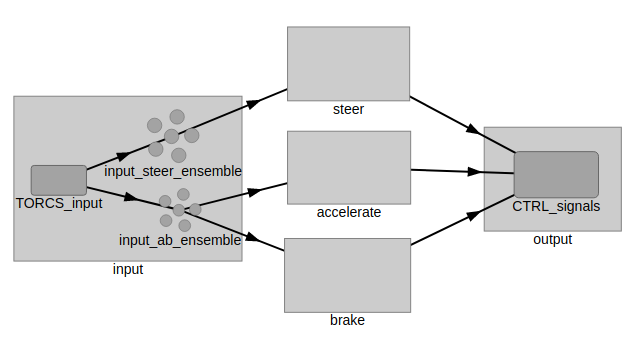
\includegraphics[width=\columnwidth]{attachments/nengo_architecture.png}
	\caption{Nengo architecture with different modules. The input network contains an input node that has subscribed to the ROS topics and contains the CNN for inference of rotation angle and lateral displacement. The steer, accelerate and brake module contain one ensemble each. The output network contains an output node that publishes to the ROS topics. The gear module is not shown here.}
	\label{fig:nengo_architecture}
\end{figure}

\subsection{Controller Training}
In this work we chose a supervised learning approach for training the controller. Nengo offers two types of learning strategies: offline and online learning.
% Besides the functionality of Nengo to directly encode and decode hardcoded functions according to the NEF \cite{nef},
With Nengo deep learning \cite{nengo_dl}, an extension to implement classic deep learning methods exists as well.

\paragraph{offline learning} can be used for the classical supervised learning approach. Feature data and corresponding labels are given and Nengo uses a least squares approximation to solve for the neuron weights \cite{nef}.

\paragraph{online learning} iteratively improves the initial neuron configuration in a supervised manner during runtime. However, this requires that for every timestep during runtime a goal value has to be known for Nengo to solve for it. In our problem this is not the case. Therefore online learning is not further considered in this work.

\paragraph{Nengo deep learning} allows to train classical deep learning methods e.g. feedforward neural networks with backpropagation and then implement the learned nets into Nengo. \\
This work focuses on a mixture of hard coded functionality and offline learning.

\subsection{Evaluation metric}
To evaluate the controller's performance, we used the following two metrics: Firstly, we investigate if the controller is able to finish one lap in a reasonable time and how fast he is compared to the default driver. Secondly, we judge the overall robustness of the controller. For this we observe the actual controller during driving and evaluated how stable he drives, e.g. how close he actually drives to the edge of the street.

\subsection{Data Sources}
\paragraph{TORCS-ROS default driver}
The first and easiest to acquire is the default TORCS-ROS driver \cite{mirus_torcs-ros_2017}. The advantage of this driver is that he drives a maximum speed of \SI{149}{\km\per\hour} and drives very carefully. Which means, that he always tries to stick to the middle lane of the road and brakes heavily when he comes close to a turn. We believe that this is an easy to learn and robust driving style. However, this driver is very slow, as can be seen in \autoref{tab:torcs_laptime}.
\paragraph{TORCS drivers}
Furthermore, there are several drivers that are implemented in TORCS. Those drivers have no speed limit and their driving style approximates that of a real race. The cars drive very close to the edge of the road and drive very fast through turns. We think that this is a hard to learn and error-prone driving style, because small errors lead to disastrous effects.
\paragraph{driving manually}
Finally, there is the option to drive manually. As it turns out this is really difficult with a keyboard. Because fractions of seconds on the left and right arrows lead to very strong steering behavior and almost every time lead to a full turn-around or a far deviation of the track. This leads to a manual driving style that comes close to the default driver: very slow through turns and sticking close to the road center. However, because it is possible to drive as fast as one wants and in general one achieves a smoother driving of the car, we achieve a faster time than the default driver. \\

\begin{table}[ht]
	\centering
		\begin{tabular}{ |c|c|c| } 
			\hline
			TORCS-ROS default & 85s \\
			TORCS  & 43s  \\
			manual & 69s \\
			\hline
		\end{tabular}
		\caption{\label{tab:torcs_laptime}This table compares the lap times of different driver types.}
\end{table}
Because of the above mentioned characteristics of the different driver styles, it we decided to first learn the TORCS-ROS default driver, because it seems to be the most robust one and data generation is simple.

\section{Experiments and evaluation}
\label{sc:evaluation}

\subsection{Performance comparison between inferring angles vs. inferring displacement}
For the final application, the same model is used to infer the car's displacement and its angle. During training, the loss function (MSE) and the metrics (MAE) are continueally evaluating the consolidated training performance. However, to determine the performance of predicting the individual values, two models were trained on each either predicting the angle or predicting the displacement of the car. \autoref{fig:mae-distance-vs-angle} shows the difference between angle and displacement prediction is shown. In training and validation set, the value of the displacement is in the range of -0.9 to 1.1 and the angle is in the range of -0.9 to 1.1. Thus, it can be concluded that the displacement prediction performance especially still needs to be worked on. 

\begin{figure}[ht]
	\centering
	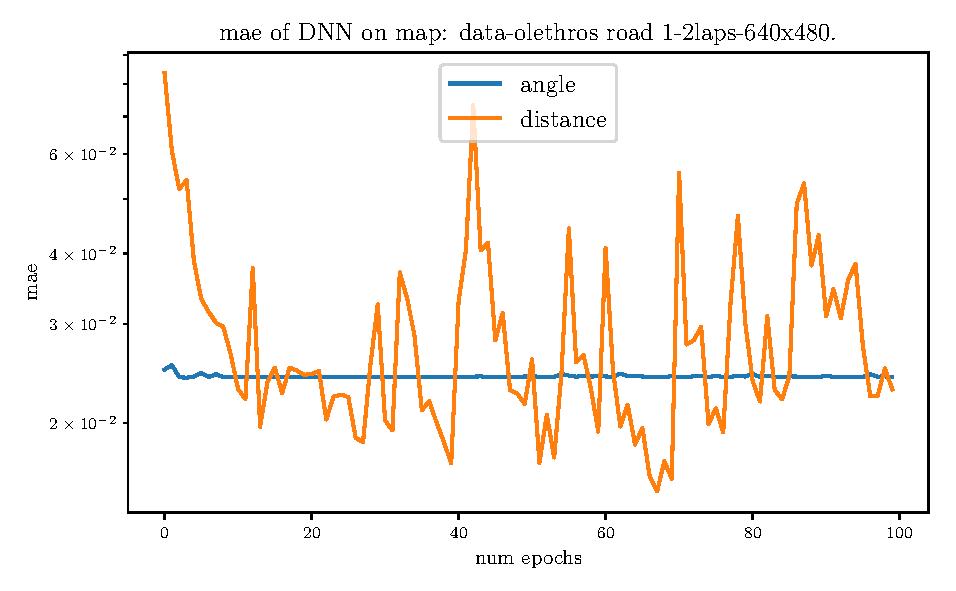
\includegraphics[width=\columnwidth]{attachments/alexnet-val_mae-angle_dist_comp-05425-86589.pdf}
	%\input{attachments/alexnet-val_mae-distance_angle_error-84095-86589-98073_-.pgf}
	\caption{Mean absolute error of two test networks trained only to predict either the displacement or angle of the car}
	\label{fig:mae-distance-vs-angle}
\end{figure}

\subsection{Prediction performance of the DNN}

\subsection{Controller performance}
Controller performance is influenced by different factors. Data composition, model capacity and forward propagation time are discussed in the following. \\
%For finetuning the results we have basically three tuning possibilities: the neuron sizes, the amount of data and the composition of tracks the data was collected from. \
In order to define the best model capacity, it is important to generalise well. The final model should not overfit nor underfit. Besides the neuron sizes for the different modules and signal encodings, also neuron composition is of interest. It is possible that one module has a more complex function and therefore needs a higher capacity to learn it's corresponding function. During testing, however, we did not see different module capacities to have a strong influence on the model. We increased the neuron sizes from a bad performing configuration until we hardly discovered any improvements on the generalisation task. We could not reach overfitting with the dataset we used, because our hardware would eventually run out of physical memory.\\
When we collected track data for training the controller, we chose tracks with slightly different shapes and turns in order to cover a vide variety of situations. We observed that small training sets would lead to overfitting of the model and for small model capacities to instable performance. Once we had enough data, the track composition did not seem to influence controller performance. \\
% Further we observed that braking needed much more neurons than accelerating and steering to work reliable. We assume the reason for this is that the braking function in the driver is highly non linear and consists also of a ABS implementation. \\
% While testing we observed that even though lower neuron counts perform equally well in lap time, they, however, performe much worse in stability. E.g. a setup with  \\
% The controller performance based on ground truth data is shown in \autoref{tab:controller_laptime}.  \\
During the testphase we observed a large variance in the data. Even when we ran tracks twice with the same configurations we obtained different track times with up to \SI{2}{\second} difference. Further, the same models showed different behaviour in critical turns. We have not yet discovered the reason for this, but we believe it has something to do with the controller frequency, which is influenced by the kernel management and other processes running on the system. Because our setup was Ubuntu 16.04 on a virtual machine, it is possible that a native host and therefore a more powerful system would show less variance. \\
% We could not test larger models, because our system ran out of physical memory in the building process (7,2 GB RAM).
% 2,800 / 3,400 - XX - xx ms -> instable, bigger laptime -> overfitting! However our model ran out of physical memory by increasing the data
% 2,400 / 3,000 / 4,500 - 2:02:91 - 1.6 ms
% 2,400 / 3,000 / 3,000 - 1:59:14 - 1.5 ms
% 2,400 / 3,000 / 3,000 - 1:59:90 - 2.6ms -> rausgehauen bei kurve
% 2:00:67 - 1.67 ms -> nicht rausgehauen
% 2:03:41 - 1.9ms
% mit 10ms signal delay 2:16:x-> 4ms prop time
% mit 10ms interrupt 2:01:59 -> 3,6 ms prop time
% mit 10ms lenkung interrupt 2:06:04 -> 3,6 ms prop time
%
% 2,000 / 2,400 / 2,400 - 2:00:41 | 0 - 1.5ms
% 2,000 / 2,400 / 2,400 - 2:01:59 | 0 - 1.47 ms
% mit 10 ms lenkung intterupt 2:04:33 -> 2,6 ms prop time
%
% 1,400 / 1,600 / 1,600 - 2:07:45 | 0.8 ms - bad performance
As already mentioned it is important to keep the control frequency high. This is necessary because with increasing model capacity, the calculation time of the controller becomes too large which lead to an instable controller. Low frequencies lead to the controller signals being already outdatet when they arrive at the car and therefore controlling becomes instable. This is especially important on computers with older hardware, which, even with native operating systems, have problems to simulate TORCS, ROS and Nengo at the same time. We observed that for average controller iteration times larger than \SI{12}{\milli\second} the controller already becomes instable. One forward propagation of the Nengo controller without a DNN takes approximately between \SI{1.5}{\milli\second} and \SI{3}{\milli\second}. This requires the DNN to have a maximum forward propagation of \SI{9}{\milli\second}. \\
Another influence on controller perfomance is the way we acquire the signal. The forward propagation of the DNN in the input node (see \autoref{fig:nengo_architecture}) leads to a delay until the calculated signal enters the SNN. As stated above, only the steering module is based on the DNN signals. In order to gain the best controller performance, we updated the range finder signals and the speed signals asynchronously. So even when the DNN was calculating the angle and displacement values, the Nengo input node still recieved updates from the ROS topics. Then, after the DNN had calculated the signals, we fed the now outdated angle and displacement values together with the most recent speed and range finder signals into the SNN. \\
As the final neuron sizes for the different modules we chose $2,000$ neurons encoding each input signal. The driving modules consist of $2,400$ neurons each. With smaller model capacities we obtained a less stable driver, while a larger model capacity did not show any improvements. \autoref{tab:controller_laptime} shows the results of the controller without the DNN, with and without \SI{9}{\milli\second} artificial interruption with asynchronous signal updates based on ground truth data input signals. \\
\begin{table}[ht]
	\begin{center}
		\begin{tabular}{ |c|c|c|c| } 
			\hline
			track &  default driver & no interruption & interruption \\
			\hline
			cg track 2  & 1:58:15 & 2:00:76 & 2:03:84  \\
			wheel 2 & 4:21:45 & 4:26:80 & 4:46:51 \\
			\hline
		\end{tabular}
		\caption{\label{tab:controller_laptime}This table compares the lap times of the controller with and without \SI{9}{\milli\second} artificial interruption against the default driver on the generalization task with ground truth data as input signals.}
	\end{center}
\end{table}
To elaborate the effects of noisy data input, we modified the input data with an additional gaussian noise with mean 0 and a standard deviation of 30\% of the signal value. We tested the model without an artificial interrupt and achieved a lap time of 2:04:14. With an artificial interrup of \SI{9}{\milli\second} we achieved a laptime of 2:30:31. Furthermore, due to the noisy data and the artificial delay the car drives in slaloms over the whole track. On the one hand this leads to a slower overall speed and therefore a faster lap time, but on the other hand the slower speed helps the car to drive in a stable through critical turns without crossing the edge of the street.
%noisy data:
% std deviation 0.3 -> 2:04:14
% std deviation 0.3 & 9ms interrupt -> 2:30:31 -> big slalom makes driver more stable in critical turns because of lower overall velocity

\subsection{Controller and DNN}



\section{Conclusion}
\label{sc:conclusion}
We identified critical factors for the controller performance and could also provide quantitative guidelines for controller stablity. A very important factor is the propagation time. A overall propagation time of less than \SI{12}{\milli\second} is desirable and puts an upper limit of approximately \SI{9}{\milli\second} on the capacity of the DNN. We further discovered that it is possible to drive the car stable, but slow, with a \SI{9}{\milli\second} propagation delay and 30\% standard deviation around the signal value. This points out a clear focus for the design of the DNN: it is more desirable to have a fast and less accurate DNN than a slow and accurate one. \\

\subsection{Outlook}
\label{ssc:outlook}
%Change training data/camera view/angle etc to improve angle prediction performance. \\
It is possible to further enhance controller performance. The biggest room for improvement is a different default driver. A slow overall speed helps immensiley to drive the car in a stable manner through the track. Furthermore, steering, accelerating and breaking also proivde room for improvement. For example the driver could use more angles of the range finder sensor to be able to drive faster through turns. Another improvement possibility is to merge the accelerating and braking module into one module, so the controller can only either accelerate or brake. Nengo Deep Learning is an interesting approach to see if controller performance could be improved further. Also a quantitative measurement of controller stability could help in finding the optimal controller capacity. \\
It further needs to be investigated if it is possible to train a DNN that fulfills the recently discovered requirements.

% each report should include all references that you cite in the work. Make sure
% that you include all references!
\bibliographystyle{ieee}
\bibliography{bibliography}

\end{document}
